% !TeX spellcheck = fr_FR
% --- --- --- --- --- --- --- --- --- --- --- --- --- --- --- --- %

\documentclass[a4paper,12pt]{report}  % args : article, report, book 
\usepackage[utf8]{inputenc}  % encodage UTF-8 
\usepackage[french]{babel}  % choix de langue, important pour maketitle et tableofcontents
\usepackage{geometry}  % géométrie de la page 
\usepackage{hyperref}  % liens internes et externes 
\usepackage{graphicx}  % images 
\usepackage{longtable}  % tableaux 
\usepackage{fontspec}  % polices d'écriture du système 
\usepackage{tabularx}  % pour des tableaux larges 
\usepackage{lipsum}  % pour du texte 
%\usepackage{titlepic}  % pour avoir une image dans \maketitle
\usepackage{titling}  % pour utiliser \theauthor, \thedate, \thetitle 
\usepackage{datetime}  % pour que la date de \thedate soit en français 
\usepackage{float}  % paramètre 'H' dans figure pour éviter un problème avec les images 
\usepackage{amsmath} % \text dans les équations

% --- --- --- --- --- --- --- --- --- --- --- --- --- --- --- --- %

\geometry{margin = 2 cm}  % marge de 2 cm (possible d'utiliser "in" aussi)

\setlength{\parindent}{0pt}  % alinéas 
\setlength{\parskip}{.5em}

% hyperref 
\hypersetup{  
	colorlinks=true,
	linkcolor=black,
	urlcolor=blue,
	citecolor=red
}

% fontspec
\setmainfont{Bricolage Grotesque}
%\setmonofont[size=6pt]{Comic Code Ligatures} 


% --- --- --- --- --- --- --- --- --- --- --- --- --- --- --- --- %

\title{Cahier des charges fonctionnel}
\author{
	Alice LIN \\
	Thisalini RAVINTHIRAN \\
	Lilian SAFAR \\
	Djivan VARTANIAN \\
	Benjamin ZHANG \\
	Louise ZHENG \\
}
\date{\today}
%\titlepic{
\includegraphics[width=0.5\textwidth]{../Design/FichiersPoster/Logo_ESIEE.pdf}}

\begin{document}
	
%	\maketitle

\begin{titlepage}
\centering
\vspace*{9cm} 
{\LARGE \bfseries \thetitle \par}
\vspace{1cm} 
\large \theauthor \par
\vspace{0.5cm} 
\large \thedate \par
\vspace{4cm} 

\includegraphics[width=0.5\textwidth]{../Design/FichiersPoster/PDF/Logo_ESIEE.pdf} 
\vfill 
\end{titlepage}

%	\pagebreak

% --- --- --- --- %

%\section*{Auteurs}
%
%\begin{itemize}
%\item Alice LIN
%\item Thisalini RAVINTHIRAN
%\item Lilian SAFAR
%\item Djivan VARTANIAN
%\item Benjamin ZHANG
%\item Louise ZHENG
%\end{itemize}

% --- --- --- --- %

\tableofcontents

\pagebreak
% --- --- --- --- %

% VENANT DU GOOGLE DOC : COLLER À PARTIR D'ICI
% https://docs.google.com/document/d/1HbEzYS0UaP-KckqQrKnavtIfuLFMVqc9utsnXRt5M9c/ 

\section{Introduction}
% Contexte du projet, problématique, objectifs du robot.

Notre projet vise à développer un robot autonome capable de livrer de la
nourriture ou des boissons de la cafétéria aux personnes se trouvant à
l'ESIEE. Le robot peut se déplacer de manière fluide, mais uniquement le
long du hall.

Une plateforme web sera mise en place permettant aux étudiants et au
personnel de l'ESIEE exclusivement de passer commande en indiquant la
salle dans laquelle ils se trouvent. Via cette même plateforme, ils
pourront également suivre leur livraison en temps réel.

Ce besoin a été identifié lors d'emplois du temps
chargés, par les longues files d'attente ou juste par la
difficulté de certains étudiants à se déplacer.

Ce projet a pour but de clôturer la fin de la première année de notre
cycle ingénieur à l'ESIEE Paris. Il permet de mettre en
application l'ensemble des connaissances acquises lors
de notre formation et d'apprendre davantage sur
d'autres logiciels informatiques et électroniques.

\textbf{Problématique :} Comment concevoir un robot permettant
de livrer de la nourriture aux étudiants depuis la cafétéria ?


\section{Architecture du système}
% Revue des technologies existantes pour la livraison autonome.

\begin{figure}[H]
	\centering
	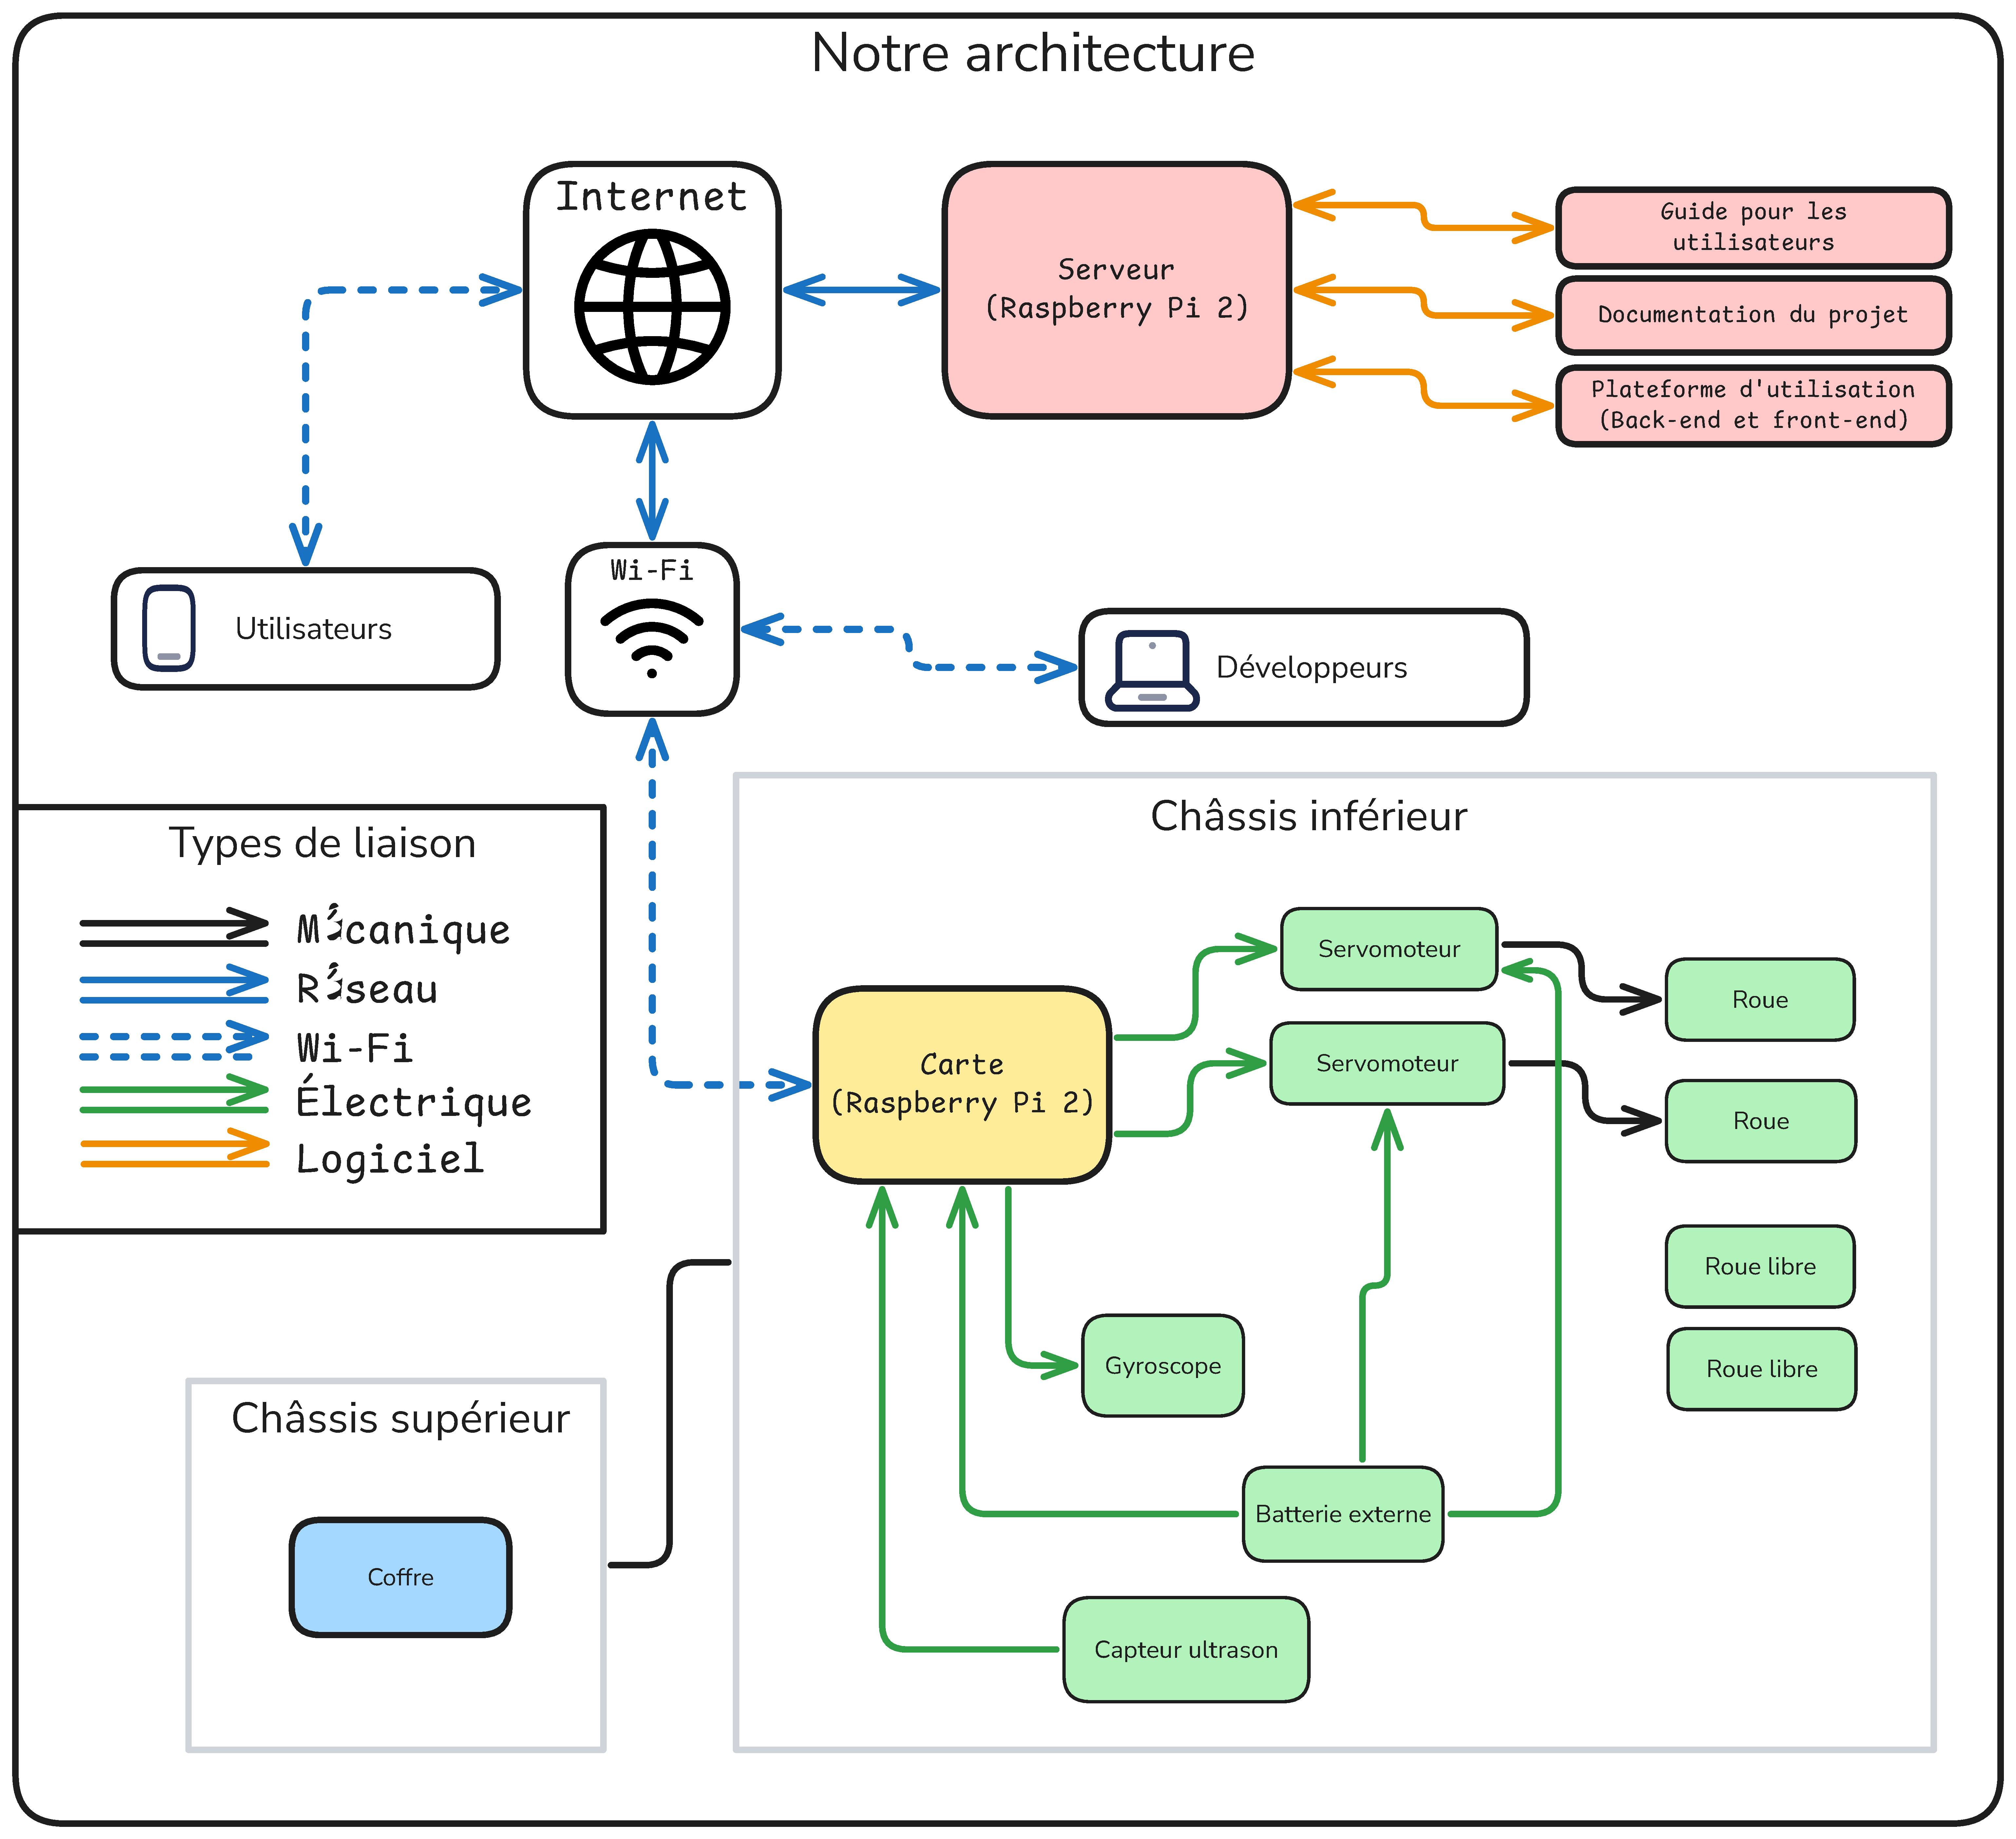
\includegraphics[width=0.6\textwidth]{./attachments/arch/2025-06-21-1200_Architecture.pdf}
	\caption{Schéma de l'architecture. }
\end{figure}

\begin{figure}[H]
	\centering
	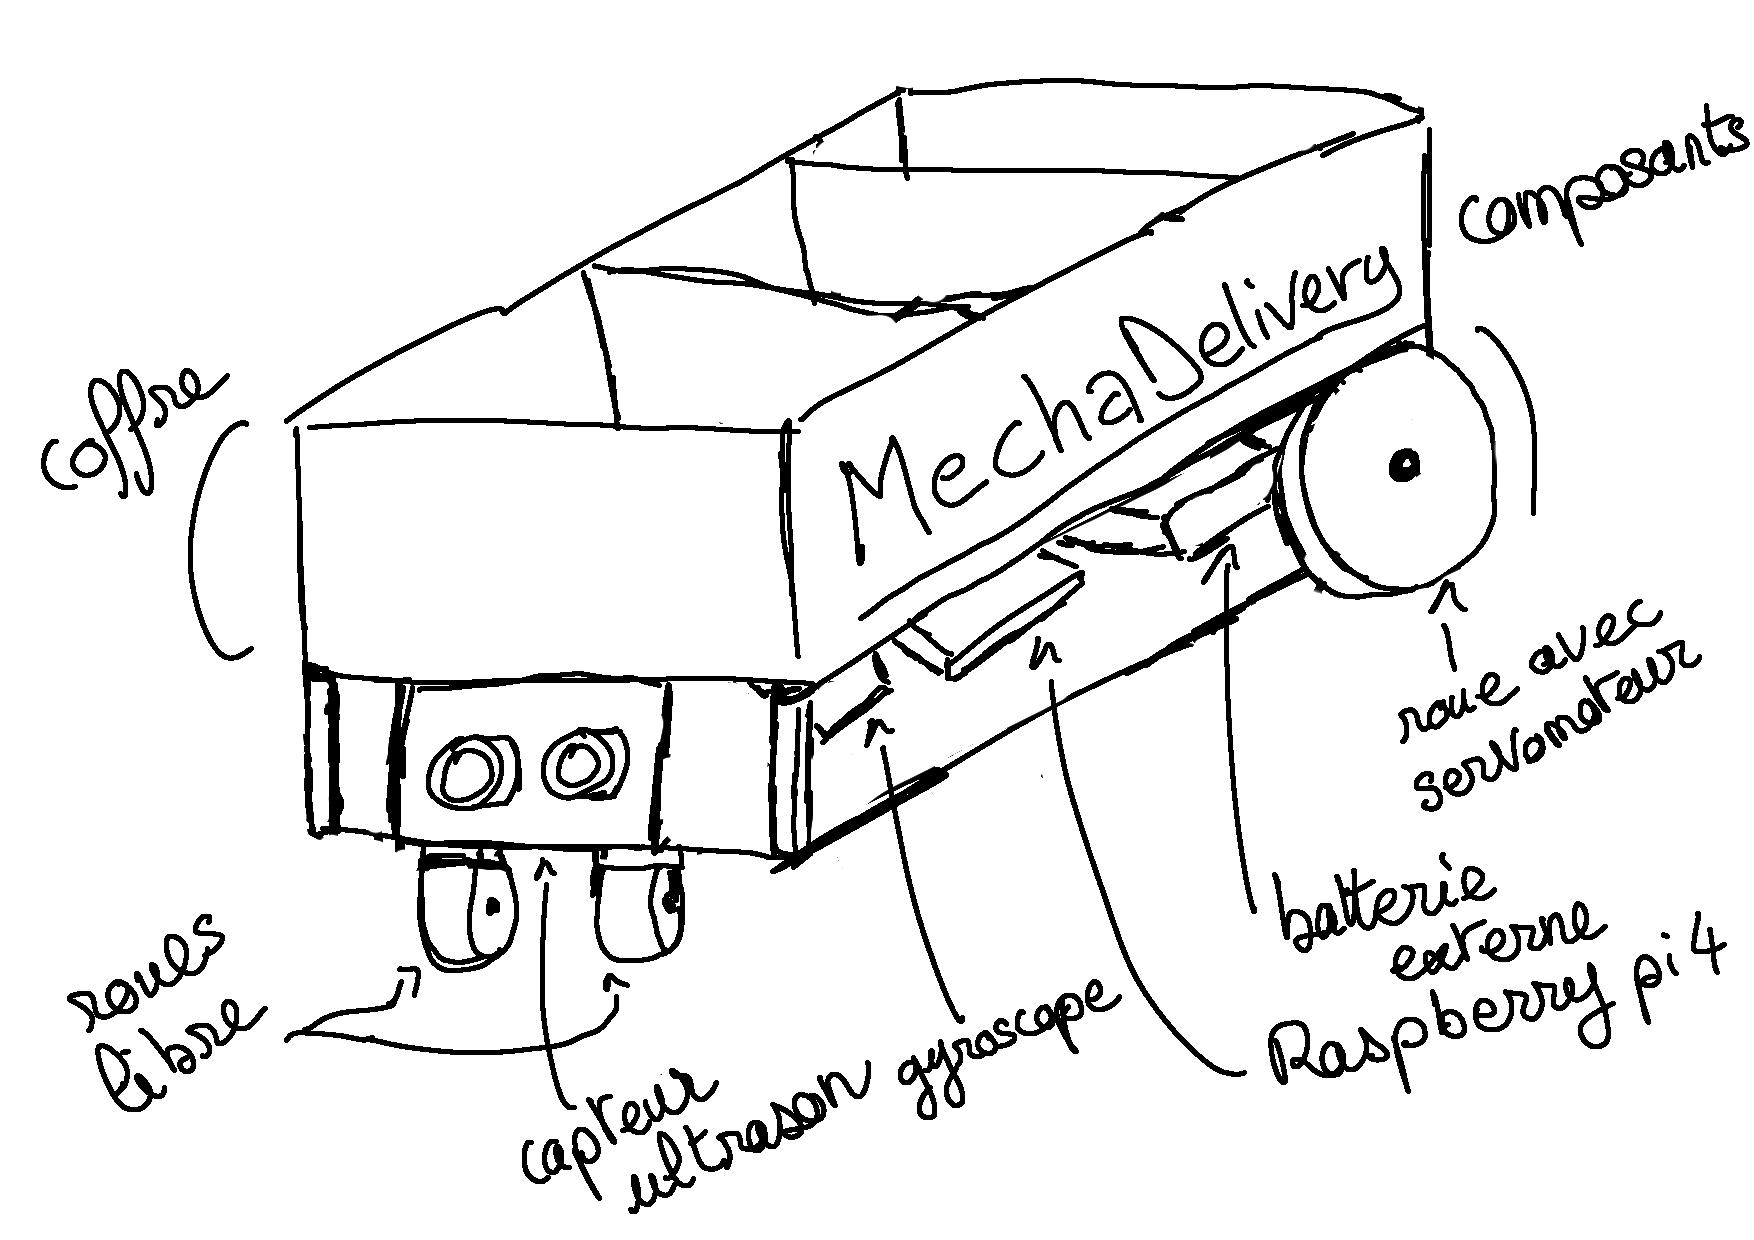
\includegraphics[width=0.6\textwidth]{./attachments/sketch.jpg}
	\caption{Schéma du prototype. }
	\label{fig:schema_proto}
\end{figure}

Liste des composants utilisés : 

\begin{itemize}
	\item
	\textbf{Raspberry Pi 4 Model B :} permet de contrôler tous les
	composants.
	
	\item
	\textbf{Module de détection US HC-SR0 :} capteur ultrason qui détecte
	les obstacles.
	
	\item
	\textbf{Servomoteur FB5311M-360 à rotation continue + feedback :}
	permet de faire tourner les roues du robot et l\textquotesingle option
	feedback permet la localisation du robot.
	
	\item
	\textbf{Paire de roulettes pivotantes à platine 
		de diamètre 40 mm (Réf 82629519) :} permet le déplacement du robot.
	
	\item
	\textbf{Paire de roues 136 mm DGR136 :} permet de déplacer le robot à
	l\textquotesingle aide des servomoteurs.
	
	\item
	\textbf{INIU Batterie Externe, 22.5 W 10000 mAh :} permet
	d\textquotesingle alimenter la Raspberry Pi 4 et les servomoteurs
	
	\item
	\textbf{Résistance 2.2 kOhm et 3.3 kOhm :} permet l'utilisation du
	capteur ultrason avec la Raspberry Pi 4.
	
	\item
	\textbf{Breadboard/PCB :} permet de relier tous les composants entre
	eux.
	
	\item
	\textbf{Module capteur LSM9DSO :} composé d'un gyroscope,
	accéléromètre, magnétomètre.
\end{itemize}



\section{Cahier des Charges Fonctionnel}

\subsection{Description des Fonctionnalités}
% Description des fonctionnalités requises (navigation, évitement d'obstacles, etc.)

{\fontsize{10pt}{12pt}\selectfont 
	\begin{longtable}{|l|l|p{4cm}|p{4cm}|p{4cm}|}
		\hline
		\textbf{Type} & \textbf{N°} & \textbf{Fonctions} 
		& \textbf{Critère de performance} & \textbf{Niveau attendu} \\
		\hline
		\endhead
		
		\hline
		\endfoot
		
		\hline
		Mécanique & F1 & Transporter de la nourriture & Capacité de charge & 3 kg de nourriture  \\
		
		\hline
		Cinématique & F2 & Se déplacer à une vitesse constante réglable & Plage de vitesse réglable & Entre \ldots{} à \ldots{}  \\
		
		\hline
		Électrique & F3 & Avoir une autonomie minimale & Durée de fonctionnement continu sans recharge & Minimum 1 h  \\
		
		\hline
		Logiciel & F4 & Navigation autonome & Itinéraire sans rechargement & \\
		
		\hline
		Mécanique & F5 & Se déplacer de manière stable & Tenue de cap en ligne droite & Pas de déviation significative pendant le trajet (à préciser) \\
		
		\hline
		Informatique & F6 & Circuler en sécurité dans l'établissement & Capacité à contourner des obstacles & Doit éviter humains, murs et objets  \\
		
		\hline
		Informatique & F7 & Détecter les obstacles & Type de détection & Détection fiable pour éviter les collisions \\
		
		\hline
		Mécanique & F8 & Sécuriser la nourriture dans le coffre & Coffre verrouillé mécaniquement & S'ouvre seulement par l'intervention humaine (bouton poussoir, écran)  \\
		
		\hline
		Mécanique & F9 & Assurer la stabilité dans le coffre & Compartimentage adapté & 3 zones : boissons, sandwichs, vide. Le nombre à fixer \\
		
		\hline
		Informatique & F10 & Avoir un site web intuitif pour contrôle utilisateur & Interface simple et claire & Navigation intuitive, accès rapide aux commandes \\
		
		\hline
		Informatique & F11 & Commander le robot via interface web & Contrôle à distance & Envoi d'ordres depuis le site (start/stop) \\
		
		\hline
		Informatique & F12 & Avoir un retour d'information depuis le robot & Données visibles en temps réel & Position, statut, livraison en cours ou terminée, batterie \\
		
	\end{longtable}
}

\subsection{Contraintes Techniques}
% Contraintes techniques (dimensions, poids, autonomie, etc.)

{\fontsize{10pt}{12pt}\selectfont 
	\begin{longtable}{|l|l|p{4cm}|p{4cm}|p{4cm}|}
		\hline
		\textbf{Type} & \textbf{N°} & \textbf{Fonctions} 
		& \textbf{Critères de performance} & \textbf{Niveau attendu} \\
		\hline
		\endhead
		
		\hline
		\endfoot
		
		\hline
		Électrique & T1 & Avoir une batterie adaptée pour l'autonomie &
		Autonomie énergétique & ≥ 1 heure d'alimentation continue \\
		
		\hline
		Cinématique & T2 & Avoir des moteurs adaptés à la charge totale &
		Vitesse fluide & à définir \\
		
		\hline
		Mécanique & T3 & Avoir des roues pouvant supporter la charge & Capacité
		de roulement sous charge & Doivent supporter ≥ charge totale à définir \\
		
		\hline
		Mécanique & T4 & Avoir un coffre assez grand & Volume utile de stockage
		& H = 25 cm, Lg = 40 cm, l = 45 cm \\
		
		\hline
		Logiciel & T5 & Avoir un capteur performant & Portée de détection avant
		& Capteur d'ultrasons : portée de 2 cm à 4 m  \\
		
		\hline
		Mécanique & T6 & Avoir un châssis solide & Résistance mécanique &
		Doivent supporter ≥ \ldots{} kg sans déformation \\
		
		\hline
		Électronique & T7 & Avoir une carte microcontrôleur adaptée & Capacité
		de pilotage & Capacité de pilotage \\
		
		\hline
		Électronique & T8 & Avoir une carte de contrôle double moteur DC &
		Nombre de canaux / compatibilité & Alimenter les moteurs et relier à la
		carte microcontrôleur. \\
		
	\end{longtable}
}



\section{Partie théorique}
Sur le repository à l'adresse \texttt{LRSVZZ-2025/docs/Hardware/Théorique.md}

\pagebreak


\section{Partie matérielle}
Pour assembler chaque composant voici un document qui nous sera très utile tout le long. 

\begin{figure}[H]
	\centering
	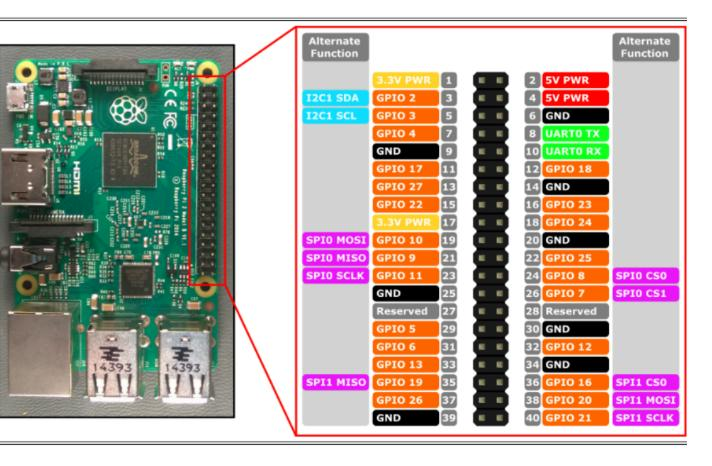
\includegraphics[width=0.6\textwidth]{./attachments/raspberry_pi_pin_map.jpg}
	\caption{Pins d'une Raspberry Pi. }
\end{figure}

\subsection{Gyroscope}

\begin{figure}[H]
	\centering
	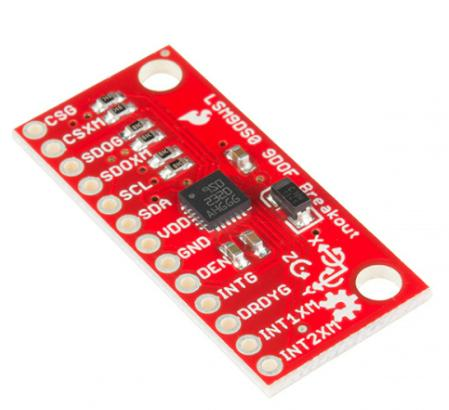
\includegraphics[width=0.3\textwidth]{./attachments/gyroscope.jpg}
	\caption{Gyroscope LSM9DS0.}
	
\end{figure}

Ce composant est un capteur 9 axes, 
composé d’un gyroscope 3 axes (mesure la rotation du robot), 
d’un accéléromètre 3 axes (la vitesse du robot) 
et d’un magnétomètre 3 axes (agit comme une boussole). 
Il va nous permettre de savoir si notre robot fait 
bien face à son point d'arrivée, s’il a assez tourné… 

Le gyroscope est alimenté en 3.3V et peut communiquer via I2C qui est un protocole de communication permettant à des appareils électroniques d’échanger des données avec le Raspberry. 

Voici les câblages à effectuer :

\begin{itemize}
	\item Relier la broche VDD du capteur à une broche 3.3V
	\item Relier la broche SDA du capteur au PIN3 
	\item Relier la broche SCL du capteur au PIN5 
	\item Relier la broche GND du capteur à une broche GND
\end{itemize}

avec : 

\begin{itemize}
	\item la broche SDA (Serial Data Line) : c’est par cette broche que les données passent (rotation, vitesse, direction absolue du robot)
	\item la broche SCL (Serial Clock Line) : Elle donne le rythme de communication (des transferts de données)
\end{itemize}


\subsection{Capteurs d’obstacle (LiDAR et ultrason)}

Pour la détection d’obstacles, nous étions d’abord partis sur l’utilisation d’un capteur LIDAR.

\begin{figure}[H]
	\centering
	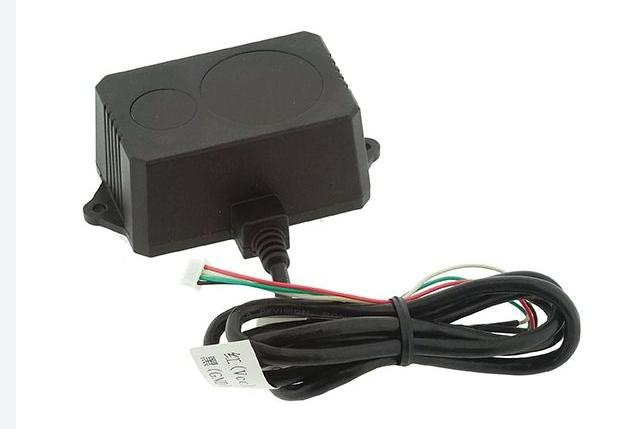
\includegraphics[width=0.3\textwidth]{./attachments/capteur_lidar.jpg}
	\caption{LIDAR Benewake TF02.}
	
\end{figure}

Le LIDAR envoie un rayon laser infrarouge en permanence, lorsque ce rayon touche un objet, il est réfléchi et revient vers le LIDAR. Le capteur va donc mesurer le temps (qu’on appelle time of flight) que le rayon à mis pour revenir, et connaissant la vitesse de la lumière, on pourra avoir la distance de l’objet qui a réfléchi le rayon infrarouge. 

Ce dispositif peut détecter des objets de 0.4 à 22 mètres en intérieur avec un angle de 3° (quasi du mono-point) et une précision de 1 à 5 cm lorsque l’objet est à moins de 10 mètres et 5 à 10 cm lorsque l’objet est entre 10 et 22 mètres. 

Le LiDAR est alimenté en 5V et délivre une tension de sortie de 3.3V. 
Il communique via UART qui est un protocole de communication série qui permet à deux appareils de s’échanger des données bit par bit sur une ligne de transmission avec le Raspberry.

Voici les câblages à effectuer :

\begin{itemize}
	\item Le fil rouge du capteur sur une broche 5V PWR 
	\item Le fil noir du capteur sur une broche GND
	\item Le fil vert (RX du LIDAR) sur le PIN8
	\item Le fil blanc (TX du LIDAR) : sur le PIN10
\end{itemize}

avec : 

\begin{itemize}
	\item Le fil TX du capteur : c’est le fil qui envoie les données => le Raspberry va donc recevoir les données via sa broche UART0 RX
	\item Le fil RX du capteur : c’est le fil qui reçoit les données => le Raspberry va envoyer les données via sa broche UART0 TX
\end{itemize}

Après câblage et lancement du programme du LiDAR (que nous allons évoquer par la suite), nous n’avions aucune donnée. Ne trouvant pas la réelle source du problème (potentiels problèmes de fils, code…), nous sommes passés à un autre capteur d’obstacles : le capteur ultrason HC-SR04. 

\begin{figure}[H]
	\centering
	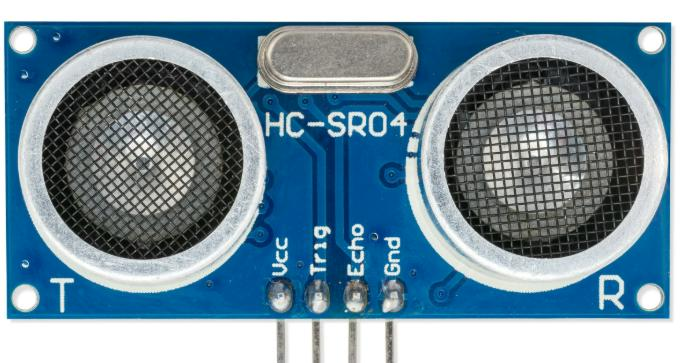
\includegraphics[width=0.3\textwidth]{./attachments/capteur_ultrason.jpg}
	\caption{Module de détection US HC-SR04.}
	\label{fig:capteur_us}
	
\end{figure}



Le module HC-SR04 permet de détecter la présence d’objets se trouvant devant lui en utilisant la réflexion des ultrasons. Le transmetteur du capteur va émettre un signal ultrason qui sera réfléchi s’il y a un objet se trouvant devant le capteur. Ce signal sera réfléchi et détecté par le récepteur du capteur. Le capteur va donc pouvoir calculer la durée entre l’émission et la réception du signal, permettant de calculer la distance entre le capteur et l’objet ayant réfléchi le signal ultrason. 

C’est le même principe que pour le LiDAR. 
En revanche, ce dispositif peut détecter des objets entre 2 à 400 cm, sa portée de détection est beaucoup plus petite que pour le LiDAR (4 mètres max vs 22 mètres max). Mais, le HC-SR04 peut détecter des objets dans un angle de 30° maximum (angle 10 fois plus grand que pour le LiDAR) avec une précision de +-3mm (plus précis que le LiDAR).

Donc, à défaut d’avoir une portée de détection d’obstacles grandement réduite, donc une moins bonne anticipation des obstacles par notre robot (pour qu’il se prépare à tourner, à contourner l’obstacle…), on est sûr qu’aucun objet ne peut perturber le déplacement de notre robot (avec un rayon infrarouge mono-point, on aurait pu passer à côté d’un obstacle par exemple sur les côtés du robot).

Ce dispositif est alimenté en 5V et sa tension de sortie 5V également. Or, il est important de rappeler que les broches d’entrée d’un Raspberry sont conçues pour du 3.3V maximum. Pour pouvoir utiliser notre module HC-SR04 correctement et ne pas endommager nos composants, il est nécessaire de mettre en place un pont diviseur de tension afin de diminuer la tension de sortie du capteur.


Voici le calcul afin d’avoir la valeur des deux résistances constituant notre pont diviseur de tension : 


Voici le calcul afin d’avoir la valeur des deux résistances constituant notre pont diviseur de tension : 

Formule du diviseur de tension : $V_{out} = V_{in} \times \frac{R_2}{R_1 + R_2}$

Application numérique : $$\frac{V_{out}}{V_{in}} = \frac{3.3}{5} = 0.66$$

$$\frac{R_2}{R_1 + R_2} = 0.66 \implies R_2 = 0.66 (R_1 + R_2)$$

$$R_2 = 0.66 R_1 + 0.66 R_2 \implies 0.34 R_2 = 0.66 R_1 \implies \frac{R_1}{R_2} = \frac{0.34}{0.66} \approx 0.5$$


Exemple de paires possibles : 
$$R_1 = 1 \, k\Omega$$
$$R_2 = 2 \, k\Omega$$

Les résistances ayant des valeurs universelles, 
nous en avons pris deux à disposition avec à peu près un coefficient de 2 entre les deux.
$$R_1 = 2.2 \, k\Omega$$
$$R_2 = 3.3 \, k\Omega$$

Voici les câblages à effectuer :

\begin{figure}[H]
	\centering
	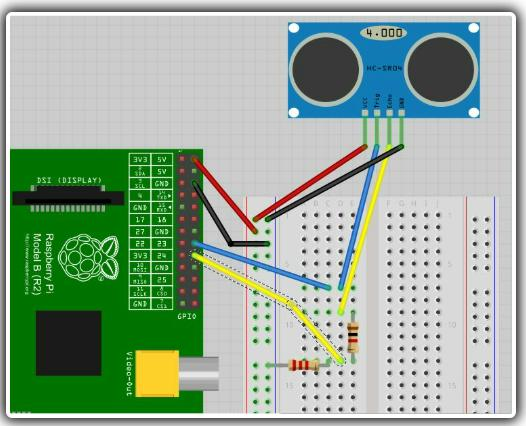
\includegraphics[width=0.3\textwidth]{./attachments/capteur_ultrason_rpi.jpg}
	\caption{Schéma du câblage.}
	
\end{figure}

\begin{itemize}
	\item La broche VCC du capteur sur une broche 5V PWR (fil rouge)
	\item La broche GND du capteur sur une broche GND (fil noir)
	\item La broche TRIG du capteur sur le PIN16 (fil bleu)
	\item La broche ECHO du capteur sur le PIN18 via le pont diviseur de tension (fil jaune) 
\end{itemize}

\subsection{Servomoteurs}

\begin{figure}[H]
	\centering
	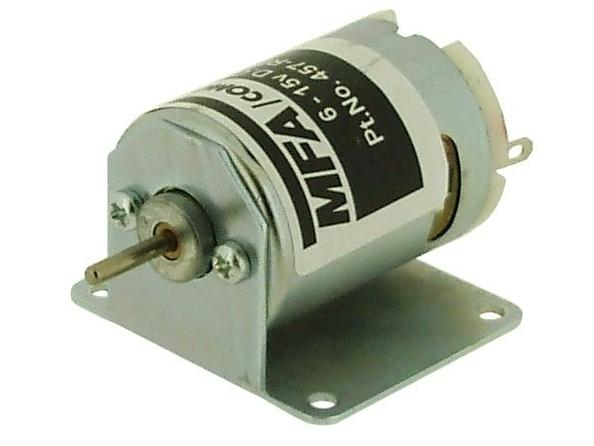
\includegraphics[width=0.3\textwidth]{./attachments/moteur_continu.jpg}
	\caption{Moteur à courant continu.}
	
\end{figure}


Pour la partie moteur, au commencement du projet nous avions des moteurs courant continu (MFA RE360), ceux que nous connaissons le mieux, une carte contrôleur double moteur cc pont en H afin de les piloter et des roues. En revanche, au moment d’assembler les roues aux moteurs, nous avons découvert que le diamètre de l’axe moteur était bien trop petit pour s’emboîter correctement dans les roues. Il y avait énormément de jeu. \\



Ensuite nous est venu l’idée d’utiliser plutôt des servomoteurs avec feedback alimentés par une batterie 6V constituée de quatre piles (1.5V chacune).

Les servomoteurs ont une meilleure précision sur le positionnement des roues que des moteurs courant continu. Et c’est plus simple de contrôler et programmer des servomoteurs (juste via un signal PWM donné par le Raspberry). De plus, les servomoteurs avec feedback ont un capteur de position intégré contrairement à des moteurs courant continu. 

Pour choisir les servomoteurs dont nous avons besoin pour notre robot, il faut les dimensionner. En attendant de les dimensionner, on a pris des servomoteurs disponibles afin de tester leur fonctionnement en amont : Parallax Continuous Rotation Servo. Tout en sachant que le fonctionnement de tout servomoteur reste le même avec des différences près (fréquence…) à modifier grâce aux datasheets. \\



\begin{figure}[H]
	\centering
	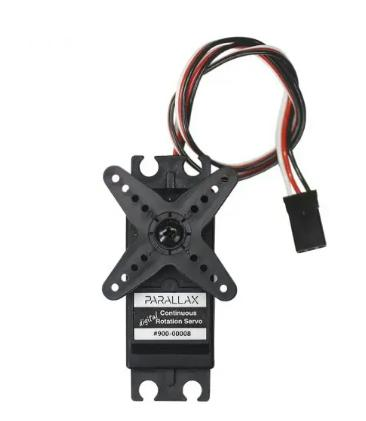
\includegraphics[width=0.3\textwidth]{./attachments/moteur_rotation.jpg}
	\caption{Parallax Continuous Rotation Servo.}
	
\end{figure}

Le Parallax Continuous Rotation Servo fonctionne en 5V. Et nous voulons qu’il soit directement alimenté par la batterie, car si on l'alimentait via le Raspberry (qui délivre bien du 5V), on avait peur qu’il soit trop sollicité et ne puisse plus être en capacité de mettre en marche correctement la partie informatique.

Donc, ayant une alimentation de 6V et un servomoteur alimenté en 5 V on doit mettre en place un régulateur de tension 5V (LM2940) pour ne pas endommager nos composants.

Voici comment nous avons mis en place notre régulateur de tension : 

\begin{figure}[H]
	\centering
	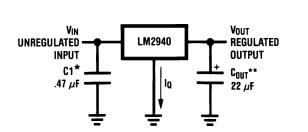
\includegraphics[width=0.3\textwidth]{./attachments/regulateur_schema.jpg}
	\caption{Schéma régulateur de tension.}
\end{figure}

\begin{figure}[H]
	\centering
	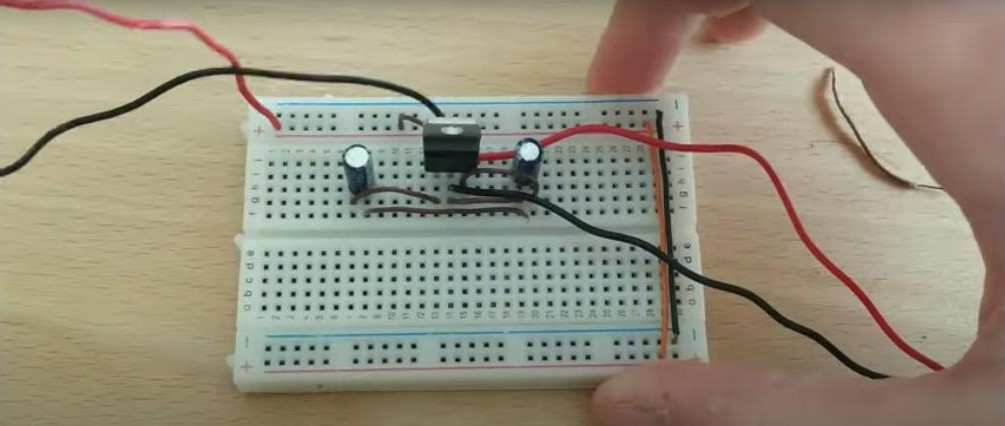
\includegraphics[width=0.3\textwidth]{./attachments/regulateur_breadboard.jpg}
	\caption{Schéma sur breadboard à faire de .}
\end{figure}




(\href{https://www.bing.com/videos/riverview/relatedvideo?&q=regulador+de+5voltios+L7805&&mid=4E46E731ADB08757CF134E46E731ADB08757CF13&mmscn=mtsc&aps=13&FORM=VRDGAR}{Vidéos Bing} 
avec à droite câble rouge et noir sur servomoteur
à  gauche, câbles de la batterie 
à ajouter câble pour relier à la masse de la Raspberry Pi)

Après plusieurs tests, pour pouvoir faire tourner la roue dans les deux sens, contrôler la vitesse de rotation… les piles se sont vite déchargées. On a donc pensé à une alternative à la cage à piles : nos servomoteurs seront alimentés par une batterie externe, la même qui alimente le Raspberry. Pour pouvoir se faire, il a fallu se procurer un fil USB A vers fils Dupont.

Le dimensionnement des servomoteurs effectué, nous sommes enfin passés à nos servomoteurs finaux (FB5311M-360). \\

\begin{figure}[H]
	\centering
	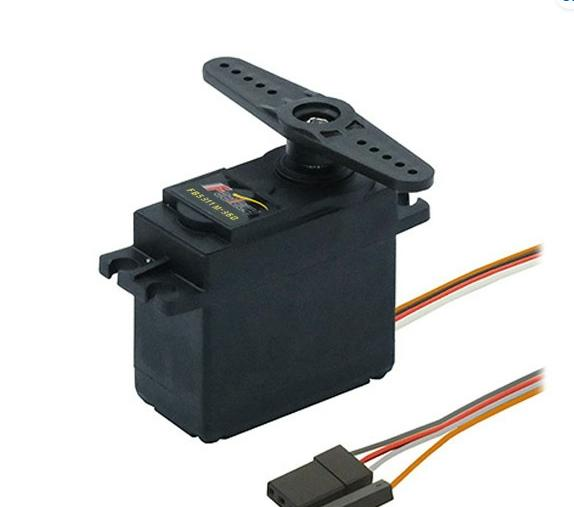
\includegraphics[width=0.3\textwidth]{./attachments/moteur_servo.jpg}
	\caption{Servomoteur FB5311M-360.}
\end{figure}

Ces servomoteurs ont un câble feedback en plus et fonctionnent de 4 à 8.4 Vcc, donc nous n’avons plus besoin de notre régulateur de tension 5V. Voici comment nous avons branché nos servomoteurs avec le fil USB A vers fils Dupont : 

\begin{figure}[H]
	\centering
	%    \includegraphics[width=0.6\textwidth]{./attachments/???.jpg}
	\caption{SCHÉMA !!!}
\end{figure}

Tout le long de l’assemblage nous avons utilisé des breadboard pour connecter les composants entre eux. Toutefois, on s’est rendu compte que certains fils Dupont se détachent, ne sont plus fixés sur le breadboard. Ce qui est assez problématique. 
Nous sommes donc passé à un PCB personnalisé puis à un veroboard qui remplacera nos breadboards.

PCB / Veroboard

\subsubsection{PCB}
Pour concevoir notre propre PCB, nous l’avons modélisé sur EasyEDA, en commençant par les branchements électroniques, puis en générant le PCB correspondant. 

\begin{figure}[H]
	\centering
	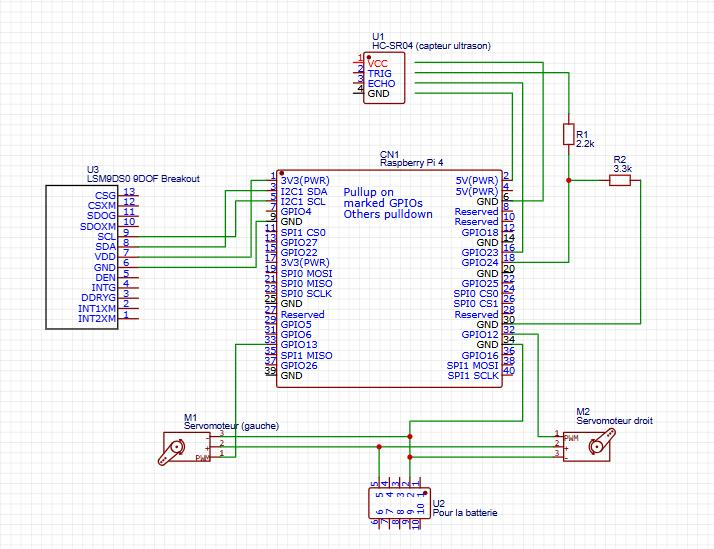
\includegraphics[width=0.5\textwidth]{./attachments/schema_elec.jpg}
	\caption{Schéma électronique.}
\end{figure}

\begin{figure}[H]
	\centering
	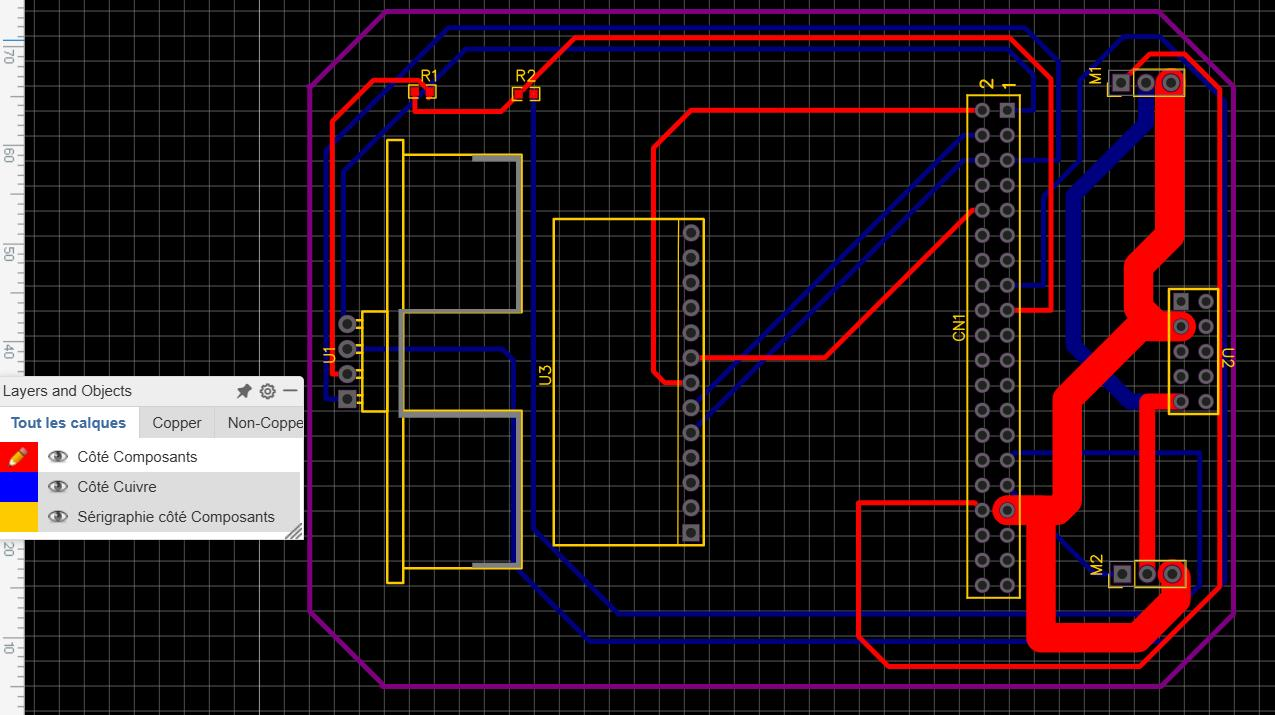
\includegraphics[width=0.5\textwidth]{./attachments/schema_pcb.jpg}
	\caption{PCB généré après avoir mis en place les wires.}
\end{figure}

Côté composants : le dessus du circuit 

Côté cuivre : le dessous du circuit



Finalement, il était trop tard pour imprimer le circuit, donc on est passé sur une Veroboard comme conseillé lors d’une réunion.

\subsubsection{Veroboard}
Sur le Veroboard, nous avons positionné tous les composants et les fils de la même manière que sur les breadboards. Contrairement à ces dernières, le Veroboard ne possède pas de circuits intégrés, il a donc été nécessaire de souder les composants et les fils.
(Schéma)



\subsection{Roues}
Comme mentionné précédemment, nous avons constaté que le diamètre de l’axe des moteurs à courant continu était trop petit pour s’adapter correctement aux roues que nous avions. Il y avait trop de jeu, ce qui rendait l’assemblage instable et peu fiable.

Face à ce problème, nous avons décidé de baser notre robot sur un servomoteur en attendant de dimensionner précisément celui dont nous aurions besoin pour la version finale. Pour nos premiers tests, nous avons utilisé un servomoteur déjà disponible. Ce servomoteur était fourni avec un kit de roues parfaitement compatibles, ce qui nous a permis de réaliser des essais pratiques rapidement.

Nous avons ainsi utilisé ce couple servomoteur-roue pour valider nos premières étapes de programmation et tester l’assemblage du robot, en lien avec notre approche théorique. Toutefois, dès le départ, nous savions que notre robot final nécessiterait des roues de plus grand diamètre pour accomplir correctement sa mission. Ces tests ont donc servi de base temporaire en attendant le choix définitif des composants.

\begin{figure}[H]
	\centering
	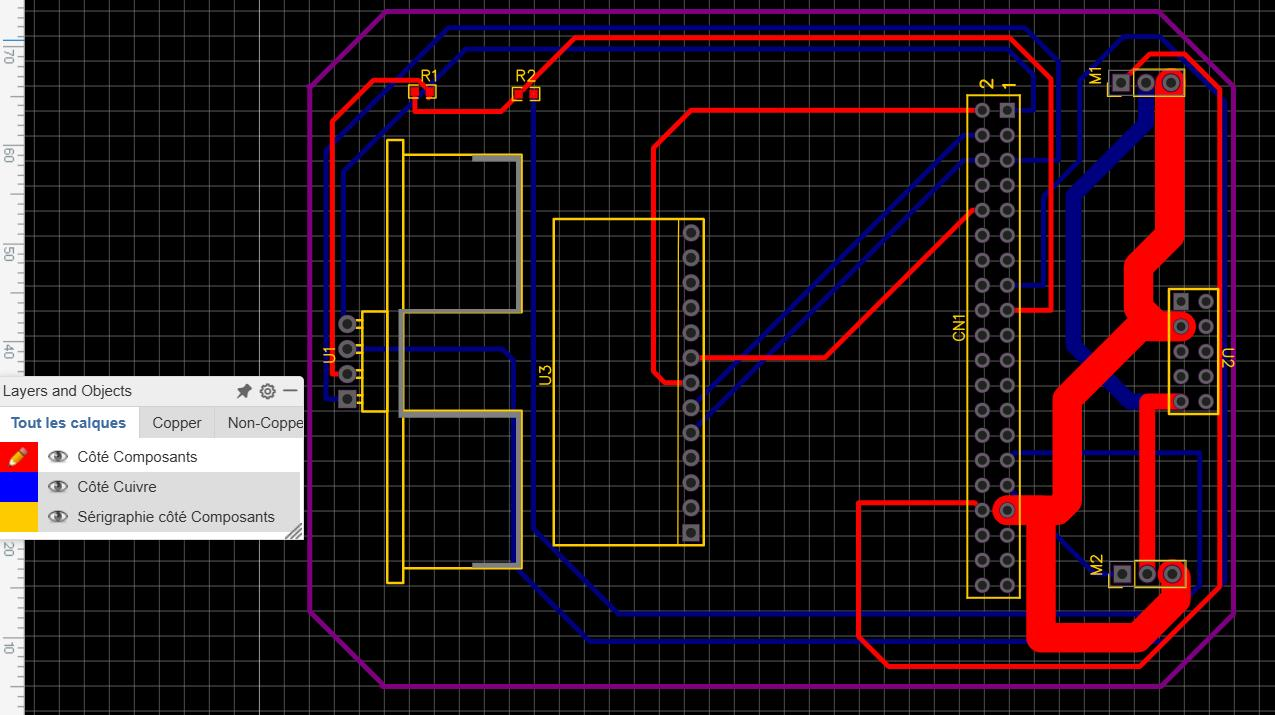
\includegraphics[width=0.5\textwidth]{./attachments/schema_pcb.jpg}
	\caption{Premières roues.}
\end{figure}

Après avoir terminé le dimensionnement des servomoteurs, nous avons souhaité passer commande des servomoteurs accompagnés des kits de roues compatibles. Cependant, seules des roues de petit diamètre étaient disponibles avec ces kits. Nous avons donc décidé de commander séparément les servomoteurs et des roues du diamètre souhaité, en pensant pouvoir les assembler nous-mêmes.

Malheureusement, à la réception de la commande, nous avons constaté que l’arbre du servomoteur n’était pas compatible avec les roues choisies. L’axe ne correspondait pas, ce qui rendait l’assemblage impossible sans adaptation.

\begin{figure}[H]
	\centering
	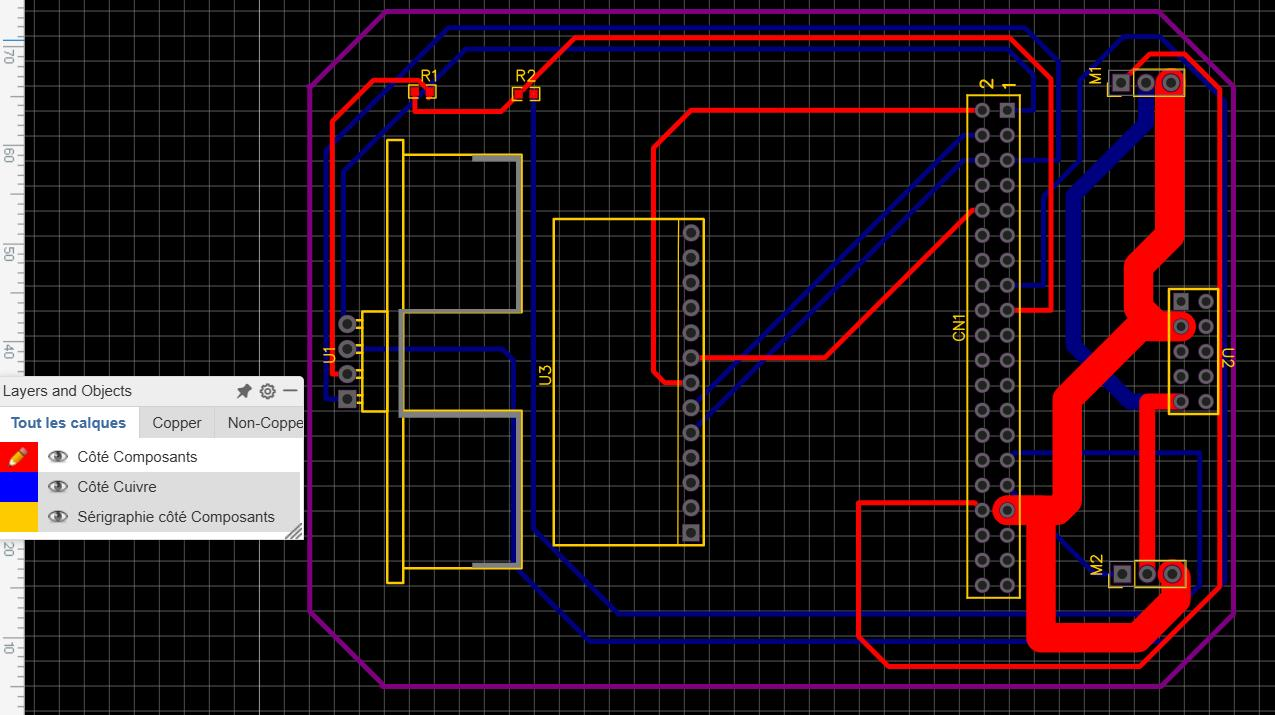
\includegraphics[width=0.5\textwidth]{./attachments/schema_pcb.jpg}
	\caption{Liens roues.}
\end{figure}


Afin de résoudre le problème d’incompatibilité entre les servomoteurs et les roues, notre première idée a été d’agrandir le trou de l’adaptateur de roue pour y faire passer l’arbre moteur et le fixer solidement. Voici le résultat obtenu :

\begin{figure}[H]
	\centering
	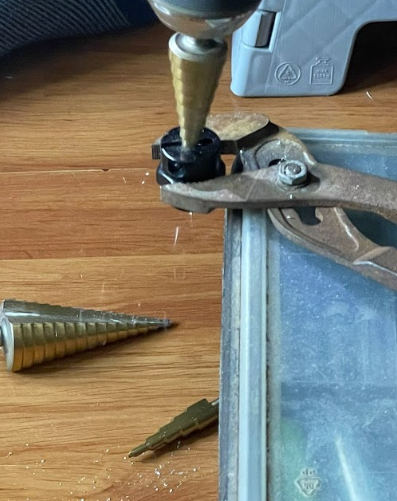
\includegraphics[width=0.3\textwidth]{./attachments/fixage-1.png}
	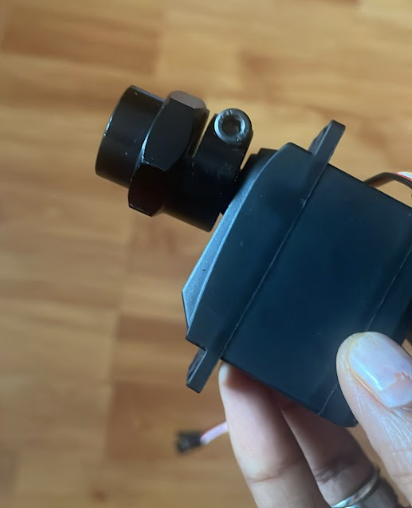
\includegraphics[width=0.3\textwidth]{./attachments/fixage-2.png}
	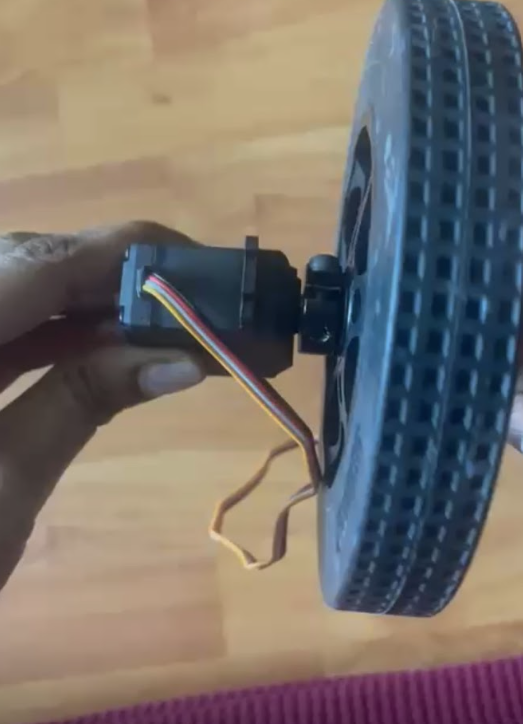
\includegraphics[width=0.3\textwidth]{./attachments/fixage-3.png}
	
	\caption{Résultat.}
\end{figure}



Après avoir fixé les servomoteurs aux roues de cette manière, nous avons réalisé un premier essai de déplacement avec notre prototype. Cependant, nous avons rapidement constaté que l’arbre moteur n’était pas suffisamment maintenu. Cela provoquait un mauvais alignement des roues, les faisant tourner de manière désordonnée, comme sur une surface glissante.

Face à ce problème, nous avons réfléchi à une autre solution plus fiable.

\begin{figure}[H]
	\centering
	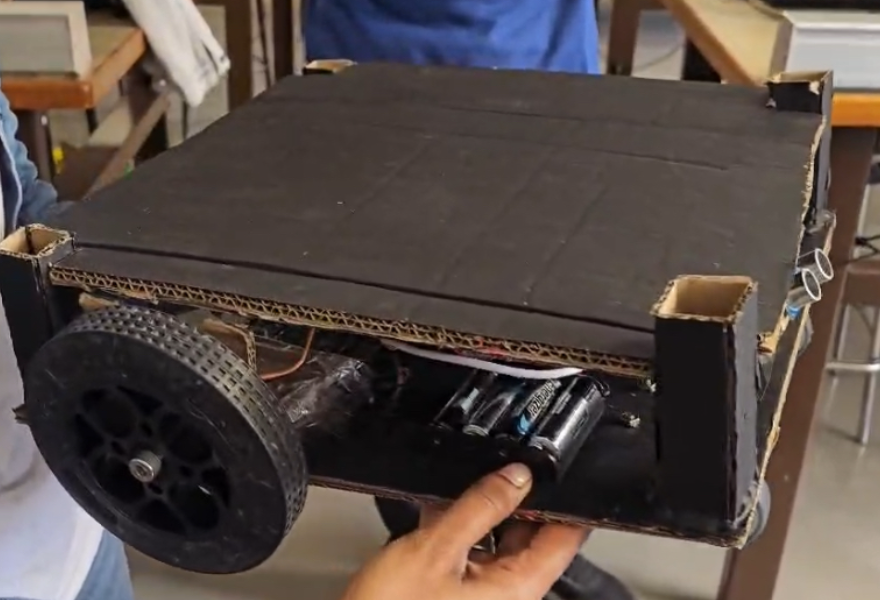
\includegraphics[width=0.4\textwidth]{./attachments/proto-photo-1.png}
	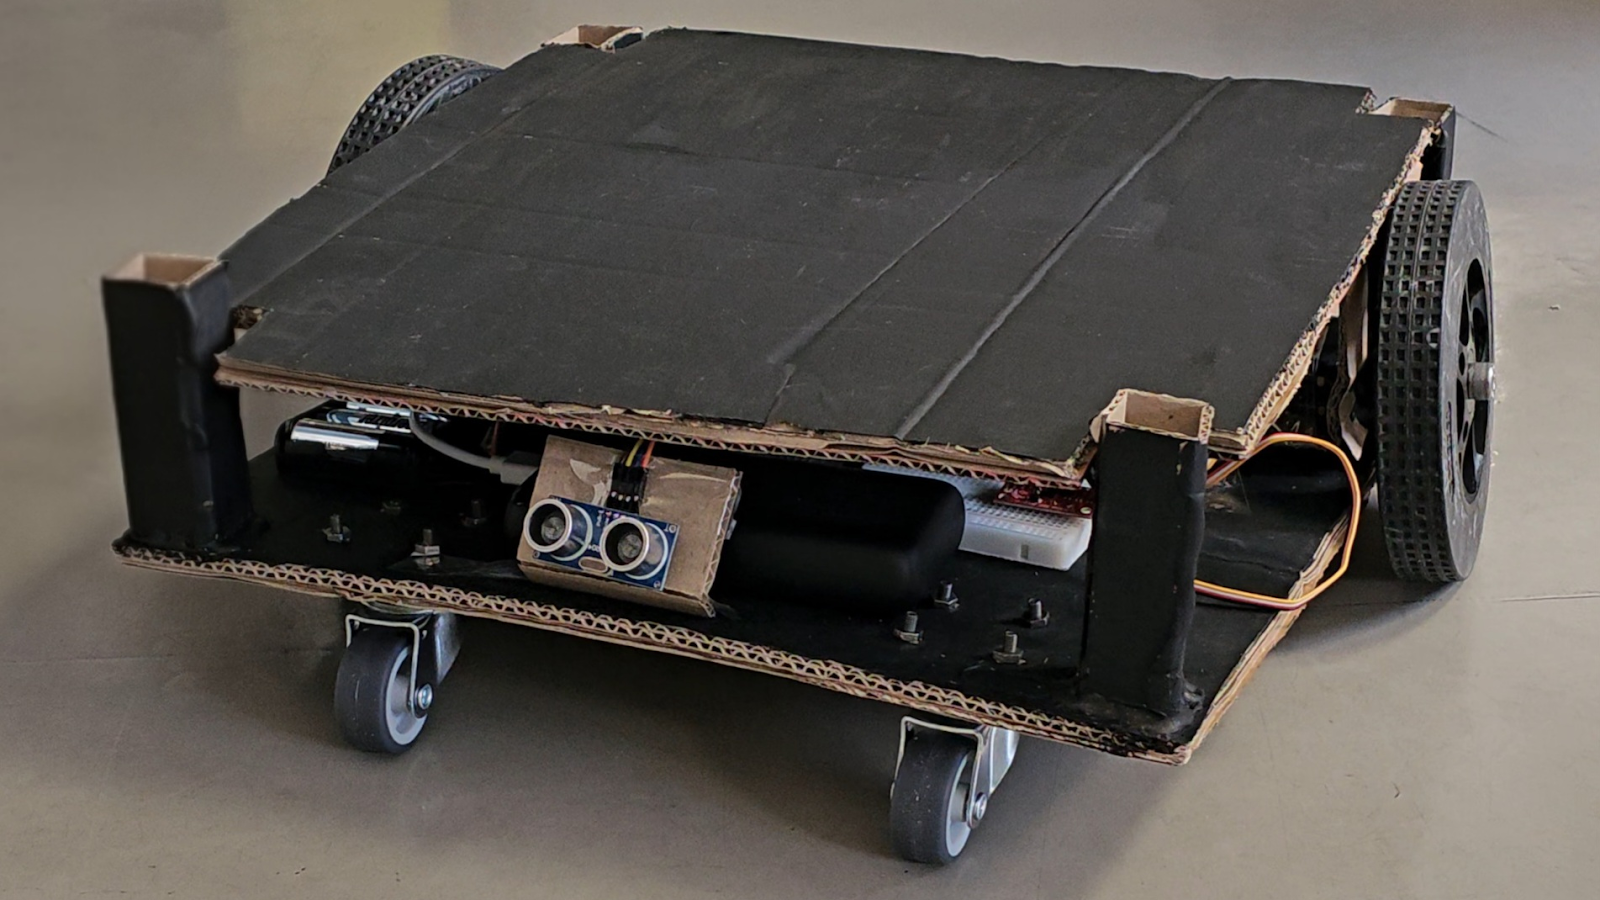
\includegraphics[width=0.4\textwidth]{./attachments/proto-photo-2.png}
	\caption{Résultat.}
\end{figure}

Après plusieurs tentatives, nous avons finalement utilisé l’équipement fourni avec les roues : des ailettes de fixation que nous avons vissées et solidement maintenues à l’aide d’écrous. Nous avons pris soin de bien aligner et fixer l’arbre moteur pour garantir la stabilité. Ensuite, nous avons monté l’ensemble sur les arbres moteurs avec précaution.

%Ensemble servomoteur-roues

\begin{figure}[H]
	\centering
	%    \includegraphics[width=0.6\textwidth]{./attachments/???.jpg}
	\caption{PHOTO !!!}
\end{figure}


\section{Structure du système}

Tout d’abord, nous avons fait un schéma du robot (\autoref{fig:schema_proto}) pour avoir un aperçu de notre projet. Nous voulions un châssis dont le coffre serait posé dessus avec des piliers, avec des compartiments qui aurait un couvercle qui s'ouvrerait automatiquement, lorsque la commande serait arrivée à destination. 

Ensuite, nous partons sur le fait d’imprimer la structure à l’aide d’une imprimante 3D. Alors nous avons en premier lieu chercher un logiciel de modélisation facile à manipuler et ensuite appris à le maîtriser. Ensuite, pour que tout le monde comprenne les outils utilisés, nous avons rédigé une documentation claire et détaillée de notre démarche sur l'outil utilisé qui est FreeCAD. Ce dernier est un logiciel de conception assistée par ordinateur open source.


\subsection{Premières impressions 3D}

\begin{figure}[H]
	\centering
	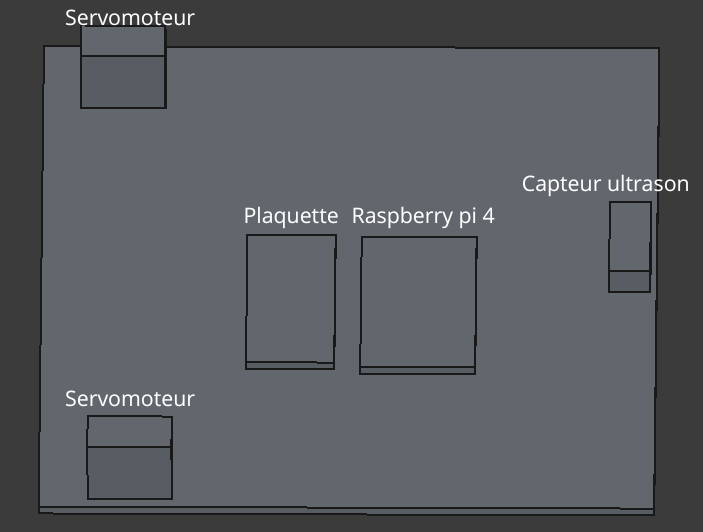
\includegraphics[width=0.4\textwidth]{./attachments/cad_planche_v2.png}
	\caption{Châssis.}
\end{figure}

\begin{figure}[H]
	\centering
	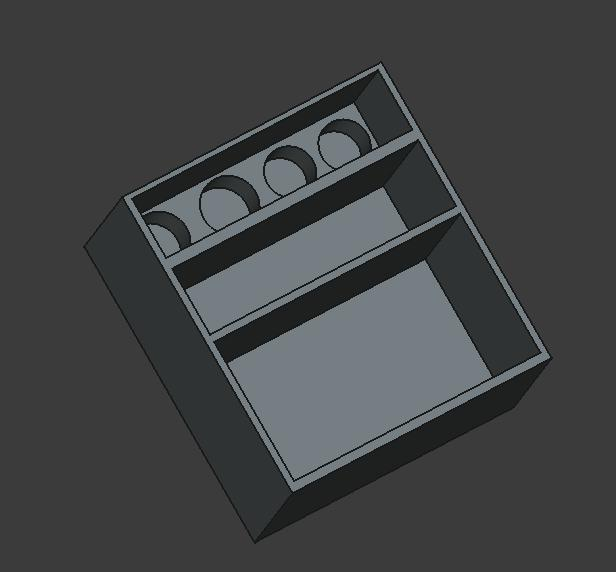
\includegraphics[width=0.4\textwidth]{./attachments/cad_coffre.jpg}
	\caption{Coffre.}
\end{figure}


Le châssis est une planche rectangulaire, que nous percerons des trous pour fixer les composants. Tandis que le coffre comporte trois compartiments, pour stocker des boissons, des sandwichs au milieu et le reste.

Après avoir modélisé les composants nécessaires, dont le châssis et le coffre. Nous nous sommes rendu compte que les dimensions des objets ne conviennent pas au plateau de l’imprimante 3D, alors nous avons pensé à diviser les différentes parties du coffre et du châssis en plusieurs morceaux. Mais cela poserait un problème pour le coffre. En effet, nous avons rapidement oublié l’idée du couvercle.

Nous voulions rester sur une structure imprimée, alors nous avons opté pour quatre petits objets en forme d'équerre et de housse qui fait le contour. Cela permettra de les accrocher ensemble et de mettre les équerres l’un sur l’autre. De ce fait, le coffre et le châssis seraient modulables et nous mettrons les composants sur les équerres et n’importe quel carton pour faire le coffre.

\begin{figure}[H]
	\centering
	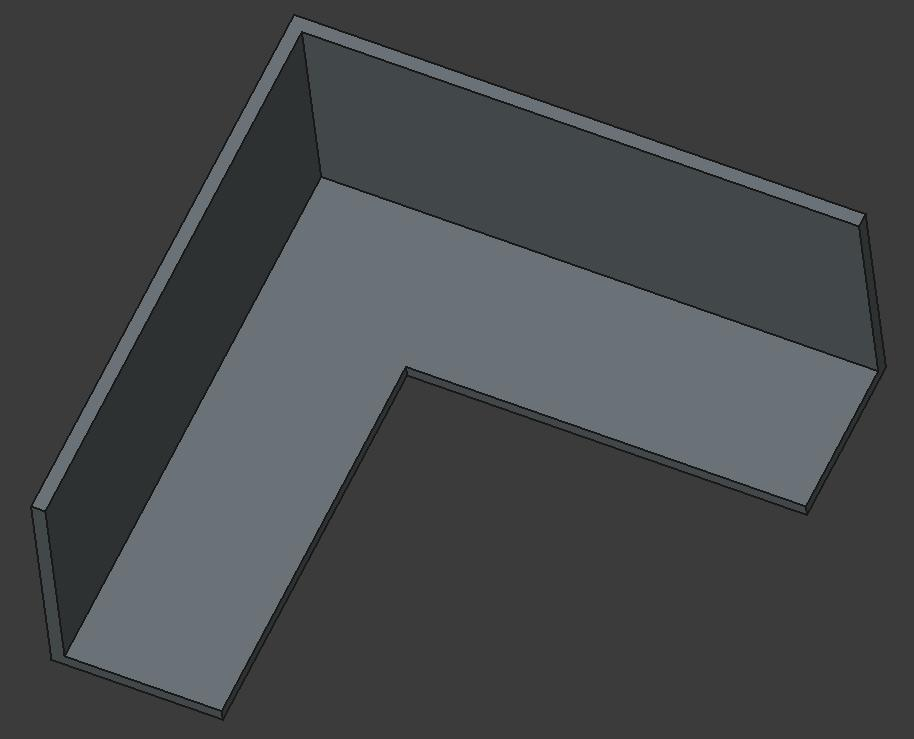
\includegraphics[width=0.4\textwidth]{./attachments/cad_equerre.jpg}
	\caption{Première équerre.}
\end{figure}

\begin{figure}[H]
	\centering
	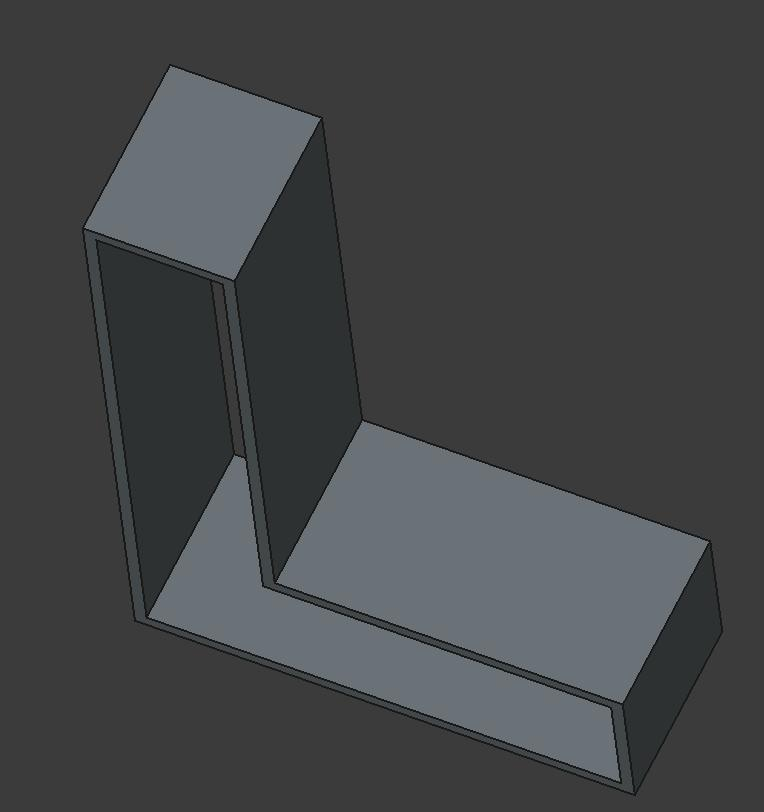
\includegraphics[width=0.4\textwidth]{./attachments/cad_housse.jpg}
	\caption{Housse.}
\end{figure}

L’équerre est assez fine pour pouvoir les empiler. Les housses sont assez large, mais de bonne taille pour bien fixer les équerres entre elles.

\begin{figure}[H]
	\centering
	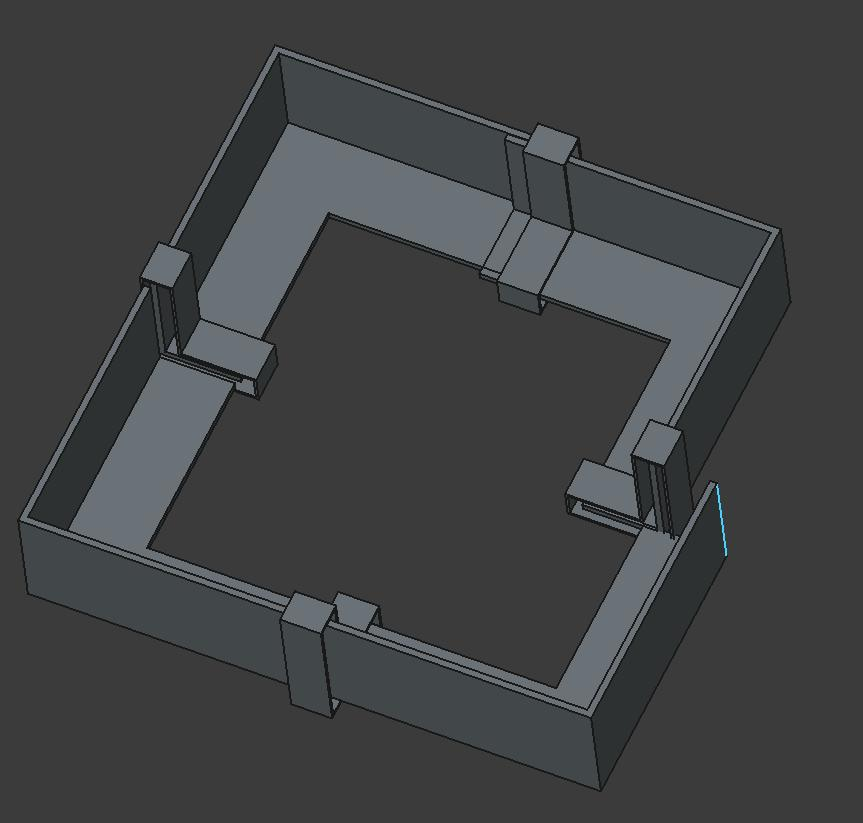
\includegraphics[width=0.4\textwidth]{./attachments/cad_assemblage.jpg}
	\caption{Ce que ça donnerait assemblé.}
\end{figure}

Après réflexions, nous avons vu qu’il y avait un problème dans nos propos. En effet, si on pose les composants sur les équerres puis ensuite un carton, ça écrase les composants.

Nous avons alors réfléchi à une meilleure solution, de faire le châssis séparément du coffre comme convenu à la base. Le châssis serait équipé de petit trou pour placer des piliers pour continuer à avoir un coffre modulable avec du carton posé dessus. 

\begin{figure}[H]
	\centering
	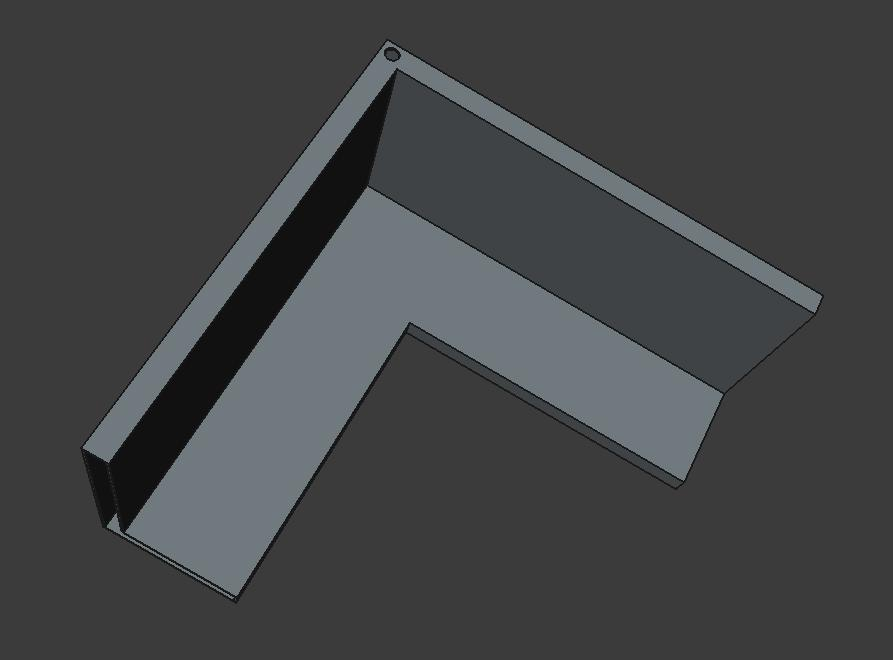
\includegraphics[width=0.4\textwidth]{./attachments/cad_equerre_v2.jpg}
	\caption{Seconde équerre.}
\end{figure}

Cette fois, les équerres seraient empilées entre elles pour éviter qu’il y ait trop d’écart entre le carton et les autres équerres, avec un trou sur le long pour pouvoir le fixer au châssis à l’aide de piliers.

\begin{figure}[H]
	\centering
	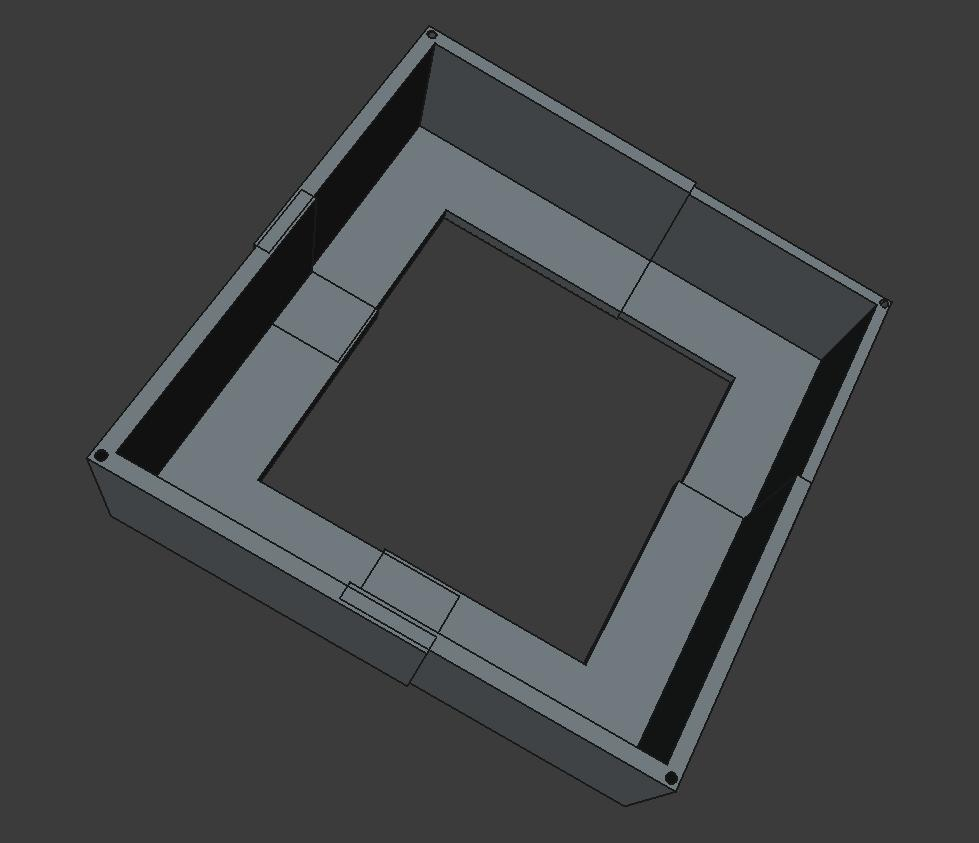
\includegraphics[width=0.4\textwidth]{./attachments/cad_assemblage_v2.jpg}
	\caption{Second assemblage.}
\end{figure}

Nous pouvons voir un aperçu avec les quatre coins assemblés, les coins ont pour but de coulisser entre elles et s’ajuster en fonction de la taille du carton choisi.

Malheureusement, cette solution n’a pas abouti, car ces coins ne conviennent pas aux temps d’impression accordés, qui dure plus d’un jour d’impression pour un seul coin.

Alors nous avons réfléchi longuement à quel matériau choisir. Nous nous sommes d’abord basés sur du bois, mais certaines planches (7 kg) dépassent le poids que peuvent supporter les roues. Nous nous sommes penchés sur le métal ou même l’acier, mais cette solution a le même problème que le bois. 

C’est alors que nous nous sommes concentrés sur le choix définitif du carton. Ce matériau est à la fois modulable, facile à manipuler, léger et facilement accessible. Il nous permet de faire et de refaire la structure sans se soucier du temps. De ce fait, nous n’avons pas la contrainte de tous les groupes à utiliser une imprimante 3D qui prend beaucoup de temps à imprimer et nous démarque par rapport aux autres groupes.

\begin{figure}[H]
	\centering
	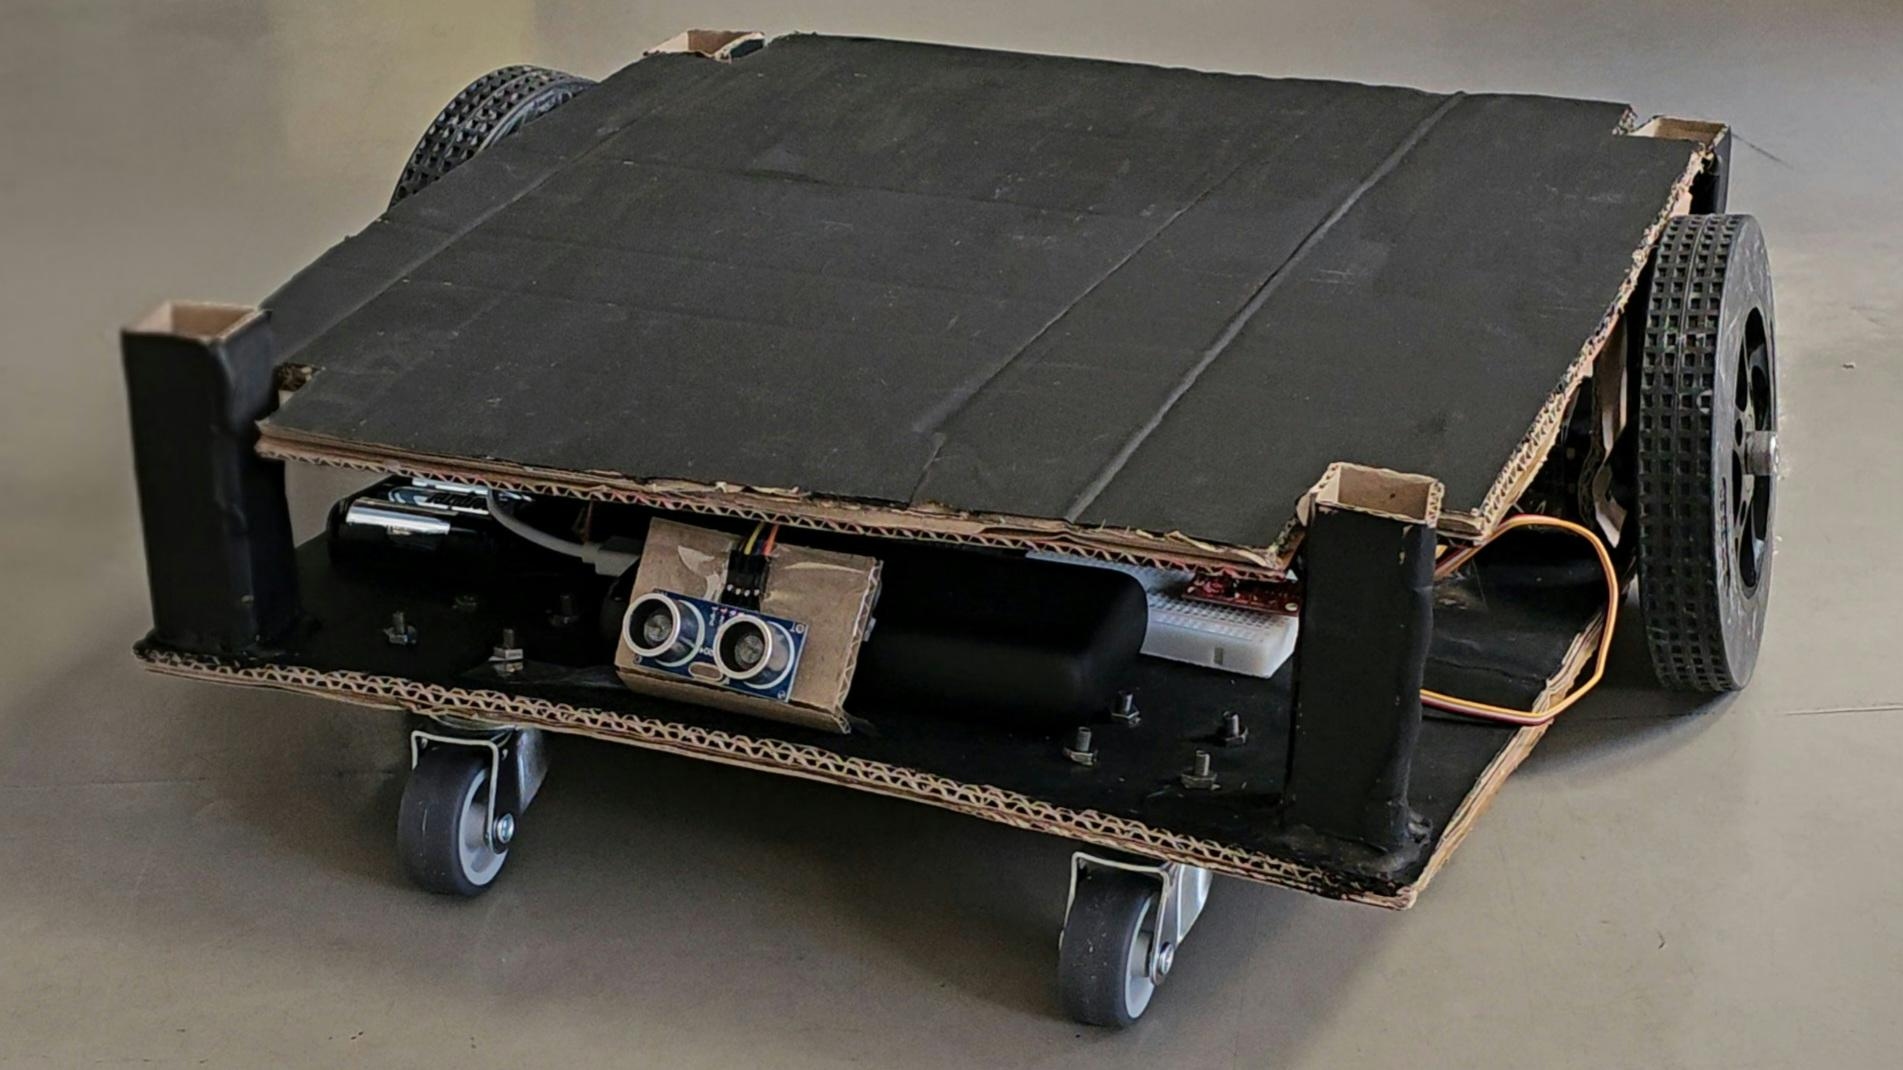
\includegraphics[width=0.6\textwidth]{./attachments/prototype_1.jpg}
	\caption{Premier prototype.}
\end{figure}


Voici le premier prototype du robot sans le coffre à l’instant. Les finitions du châssis sont plutôt négligées et le carton utilisé n’est pas très solide, nous pouvons voir que le châssis n’est pas droit. Cependant, il a été peint à la peinture et nous pouvons voir que ça couvre le fait que ce soit du carton. 

C’est pour cela que nous avons refait une autre structure avec des finitions plus propre et avec du carton beaucoup plus solide. Ensuite, nous l’avons peinte à la bombe pour avoir un rendu plus uniforme et pouvoir peindre surtout plus rapidement, ainsi éviter le temps de sèche. 

Certaines planches de cartons solides étaient assez fines, alors nous l’avons renforcé en collant plusieurs planches entre elles pour bien renforcer le châssis et supporté la force des moteurs.

\subsection{Ensemble servomoteur-roues sur le robot}
Après avoir fixé les servomoteurs aux roues, nous avons cherché un moyen de les fixer solidement sur la structure du robot, réalisée en carton. Notre première idée a été de fabriquer des équerres en forme de \textbf{L} afin de relier les servomoteurs au châssis.

Dans un premier temps, nous avons fixé les servomoteurs aux équerres à l’aide de scotch, puis attaché ces équerres au robot également à l’aide de scotch pour ce tout premier essai, sans utiliser de vis.

Cependant, nous avons rapidement constaté que ce montage manquait de stabilité : le scotch ne tenait pas bien, se décollait facilement, et ne permettait pas un bon maintien des servomoteurs.

Voici le résultat obtenu :
\begin{figure}[H]
	\centering
	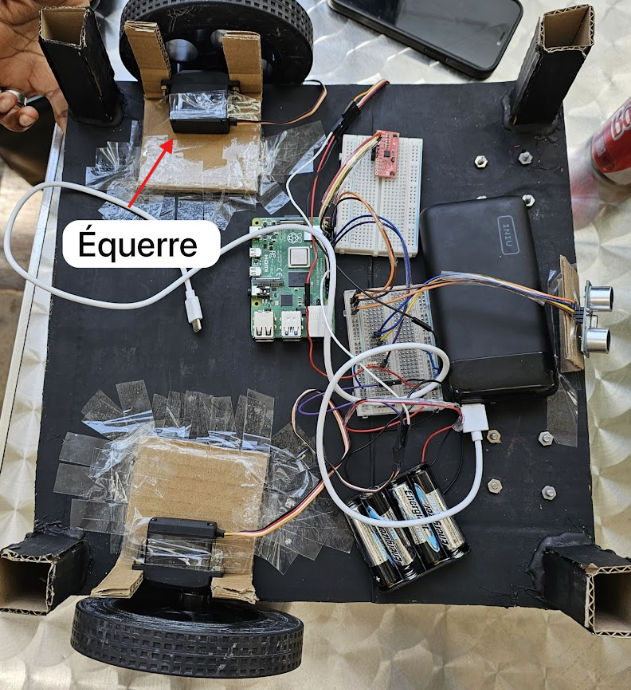
\includegraphics[width=0.6\textwidth]{./attachments/servomoteur-roues.png}
	\caption{Description.}
\end{figure}

Afin de résoudre ce problème, nous avons conçu un support en carton sur lequel nous avons fixé le servomoteur à l’aide de scotch. Ensuite, nous avons attaché ce support en carton à la structure du robot en utilisant des vis. 

\begin{figure}[H]
	\centering
	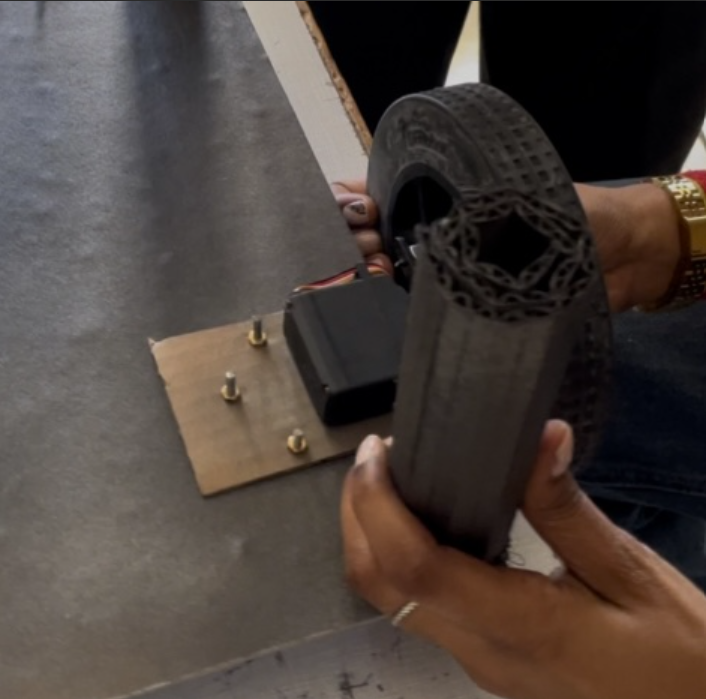
\includegraphics[width=0.6\textwidth]{./attachments/servomoteur-roues_vis.png}
	\caption{Description.}
\end{figure}

Après avoir réalisé plusieurs essais avec cette méthode, nous avons constaté que les vis ne suffisaient pas à fixer solidement le support en carton à la structure du robot. Sous le poids des roues, le carton se déformait à l’arrière, ce qui entraînait un mauvais alignement des roues.

Pour tenter de résoudre ce problème, nous avons testé différentes méthodes. Nous avons d’abord essayé d’ajouter de la colle chaude en complément des vis pour renforcer la fixation du support. Cependant, cela ne s’est pas révélé suffisamment efficace. Nous avons ensuite utilisé de la colle forte, toujours en complément des vis et de la colle chaude, afin d’obtenir un maintien plus rigide.

Malgré tous ces efforts, la fixation restait imparfaite et ne garantissait pas une stabilité suffisante pour le bon fonctionnement du robot. Nous avons donc décidé de concevoir un support imprimé en 3D, plus rigide et mieux adapté à notre besoin.

\begin{figure}[H]
	\centering
	\includegraphics[width=0.6\textwidth]{./attachments/servomoteur-roues_modèle.png}
	\caption{Modèle 3D du support.}
\end{figure}

Cette pièce agit comme un support de fixation pour le moteur sur le châssis.

Voici le résultat : 

\begin{figure}[H]
	\centering
	%    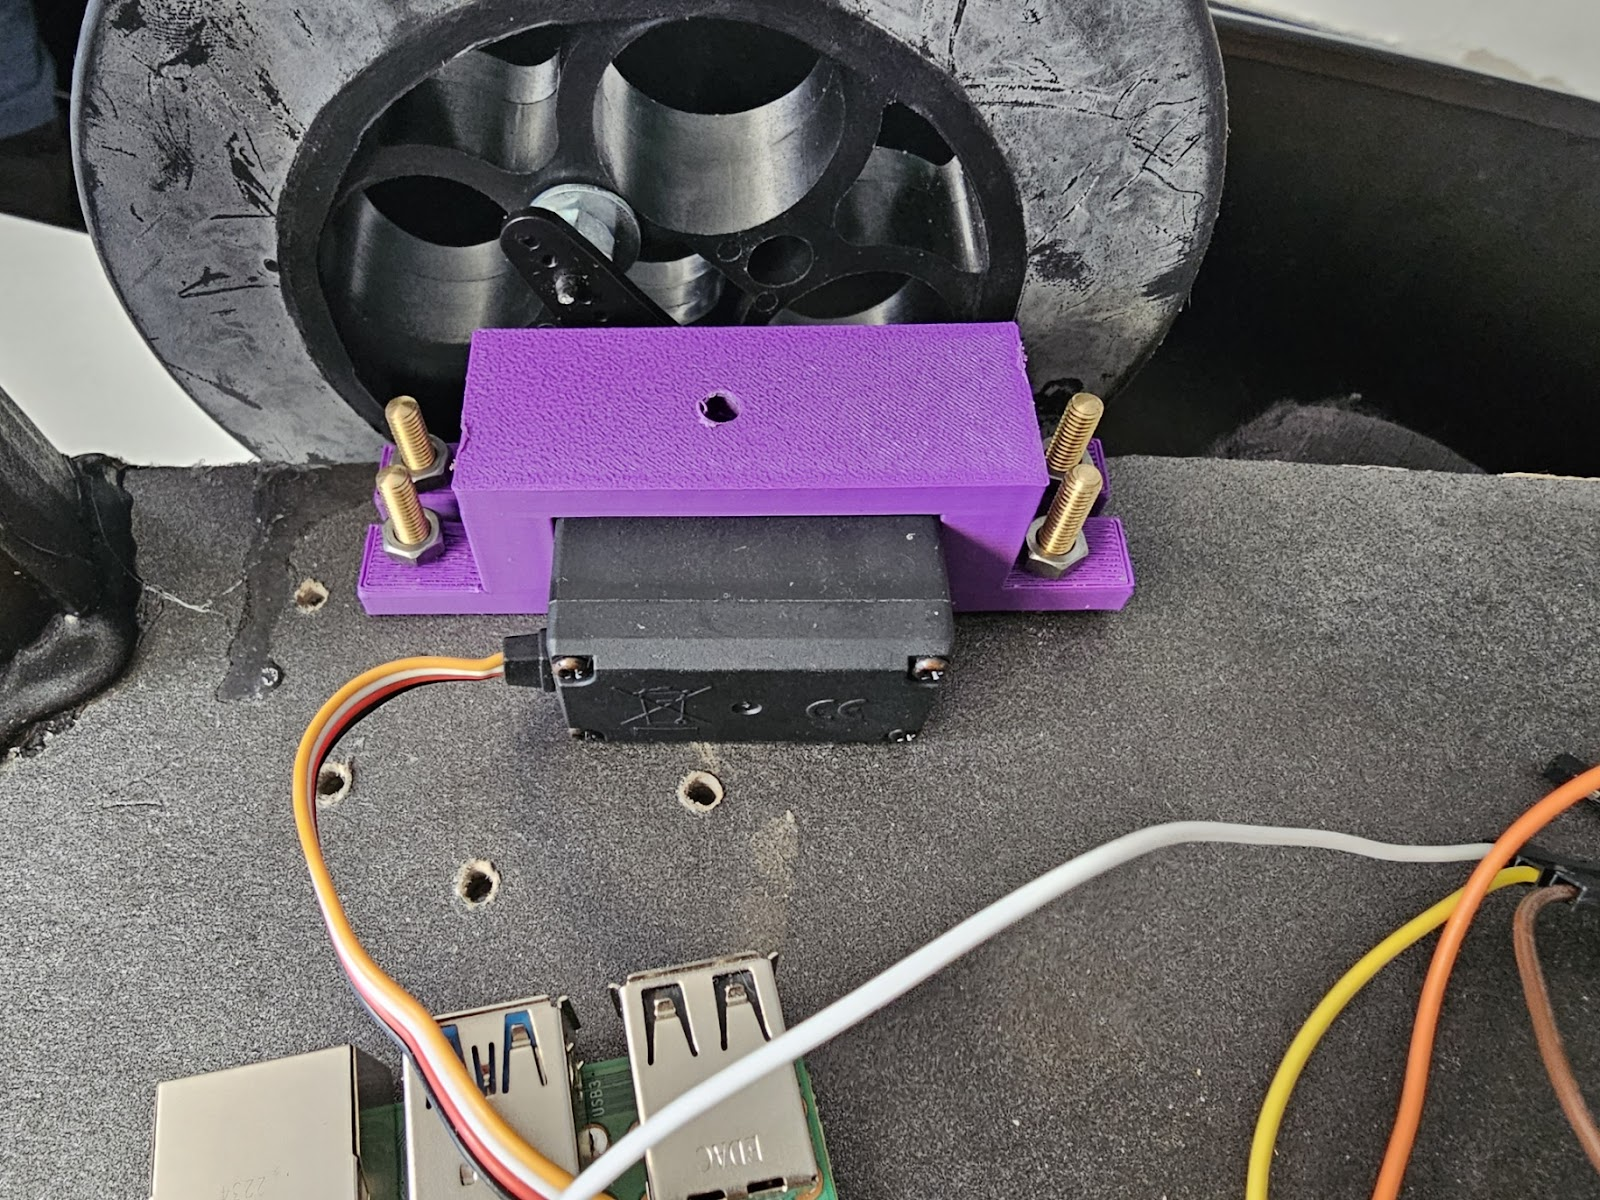
\includegraphics[width=0.6\textwidth]{./attachments/servomoteur-roues_impression.png}
	\caption{PHOTO A METTRE. \\ Version imprimée du modèle.}
\end{figure}

\section{Partie logicielle}
% Étapes de développement, utilisation de Git, défis rencontrés.
\subsection{Programmation individuelle des composants}

Gyroscope

Capteur d’obstacle (Lidar et ultrason)

Pour le LiDAR

Pour l’ultrason

Servomoteurs




Programmation du site web




\section{Gestion du projet}

\subsection{Organisation des Tâches}
% Inclure un tableau ou un graphique du rétroplanning.


\subsection{Liste des Actions Réalisées}
% Liste des actions réalisées pendant le projet.

\begin{itemize}
	\item Mettre en place les outils de suivi
	\item Choisir le modèle et la version de l'ordinateur intégré au robot
	\item Faire le rétro planning
	\item Fixer des scénarios simples pour les premiers prototypes
	\item Organiser les rôles de chaque personne de l'équipe
	\item Créer le repository pour le code et la documentation
	\item Faire la modélisation mécanique 1 (schéma cinématique + graphe des liaisons)
	\item Mise en place d'un serveur fixe 
	\item S’initier à la Raspberry Pi en découvrant ses bases et les sources d'information
	\item Configurer automatiquement la Raspberry Pi sur le réseau eduroam 
	\item Récupérer l'adresse IP de la Raspberry sur un réseau local
	\item Configurer la Raspberry sur le réseau local
	\item Créer la plateforme web qui récupère les adresses IP locales des robots
	\item Étudier le pilotage du robot (cinématique)
	\item Établir l'architecture
	\item Configurer les cartes intégrées pour la connexion à eduroam 
	\item Faire un schéma de l'ensemble du robot 
	\item Estimer le poids max du robot 
	\item Prendre en main MobaXterm pour programmer
	\item Mettre en place le cahier des charges
	\item Structurer les informations collectées et organiser les données par catégories sous forme de tableau
	\item Prendre en main les outils de modélisation 3D
	\item Choisir la version adaptée du logiciel de modélisation 3D
	\item Débuter la documentation de la partie logicielle
	\item Adapter le contenu aux standards d’un document technique ou d’entreprise (CDCF)
	\item Etudier la stabilité du robot (dynamique + asservissement)
	\item Rendre la documentation naviguable
	\item Choisir un châssis et les matériaux
	\item Mettre le cahier des charges au format systml
	\item Débuter la documentation de la partie théorique
	\item Coder le programme pour utiliser le LIDAR
	\item Mettre en place un pont diviseur de tension pour le capteur d'ultrasons
	\item Rédiger une documentation sur le processus de modélisation 
	\item Installer et prendre en main un framework JavaScript pour la création du site 
	\item Brancher le capteur d'ultrasons à la raspberry
	\item Programmer le capteur d'ultrason
	\item Faire des recherches et comparer des versions de robots existants
	\item Justifier le modèle de Raspberry Pi adapté au projet
	\item Mettre en place un lien de communication entre le frontend en JavaScript et le backend en Python
	\item Brancher le LIDAR à la Raspberry Pi
	\item Envoyer des instructions à une Raspberry Pi 4 depuis le serveur
	\item Ajouter la documentation sur la plateforme web
	\item Dimensionner le moteur + la batterie (partie dynamique)
	\item Modéliser le châssis et le coffre en 3D
	\item Déterminer le système de localisation du robot
	\item Mettre en place les moyens de communication en temps réel entre le serveur et les clients
	\item Débuter la documentation de la partie matérielle
	\item Réaliser le poster
	\item Réaliser la vidéo
	\item Permettre la manipulation des Raspberry Pi depuis le site
	\item Réaliser le châssis
	\item Positionner les composants sur le châssis (Assemblage)
	\item Contrôler les moteurs par la Raspberry
	\item Communiquer avec le capteur ultrason par la Raspberry
	\item Brancher tout les composants entre eux
	\item Choisir les moteurs et les roues
	\item Etudier la stabilité theorique du systeme 
	\item Programmer le gyroscope
	\item Mettre en relation les moteurs et le détecteur d'obstacles
	\item Décorer le châssis
\end{itemize}

\subsection{Compte Rendu des Réunions Hebdomadaires}
% Résumé des points discutés lors des réunions. 

7 Mai 2025 
Discussion de date importante et de la notation.
Approvisionnement du matériel.
Le déroulement des rendus hebdomadaires et de la soutenance.
Discussion du cahier des charges et de l'interlocuteur principal entre le suiveur et l’équipe de projet.
Discussion de l’architecture du projet.


16 Mai 2025
Discussion sur les choix matériels et logiciels.
Présentation d'un prototype de communication à distance avec la raspberry.
Évocation de la difficulté à utiliser un LIDAR pour la localisation du robot.
Discussion du scénario du projet.
Discussion du design du projet ainsi que des logiciels 3D à utiliser et imprimante 3D disponible.


28 Mai 2025
Réattribution des rôles.
Choix des matériaux et composants.
Discussion des modélisations 3D niveau technique.
Discussion niveau software, hardware et la manière dont le robot va se déplacer.
Discussion sur le déroulement de la journée des projets.


6 Juin 2025
Observation et démonstration prototype, il y a quelques problèmes.
Détails supplémentaires sur la notation.


12 Juin 2025
Discussion sur l’esthétique du software et du prototype du robot.
Discussion sur le poster et le cahier des charges fonctionnels/rapports à rendre.


20 Juin 2025
Discussion sur les problèmes de connectiques.
Déroulement de la soutenance et de la journée des projets.


23 Juin 2025




\section{Conclusion}
% Bilan du projet, perspectives d'amélioration.

Ce projet a pour but de livrer de la nourriture de la cafétéria aux personnes se trouvant à l’ESIEE en commandant depuis un site web, transporté par l’intermédiaire d’un robot sans trop se déplacer. Grâce à ce projet nous avons appris beaucoup de choses sur la construction d’un robot, notamment au niveau logiciel et matériel. La construction d’un robot et d’un site web est très longue à faire. Malgré le temps et nos connaissances moindres dans ce domaine nous avons quand même mené à bien ce projet.

Dans le futur, ce projet pourrait être amélioré de par le fait que le robot puisse prendre l’ascenseur pour livrer directement devant une salle. Faire un robot plus solide, plus propre que seulement en carton.


\section{Annexes}
% Graphiques, schémas, photos du robot, code source.
%\section{Documentation et Ressources}
% Documentation hébergée sur le serveur, liens vers les ressources.

\section{Remerciements}
Le papa de Thisalini pour son aide à plusieurs reprises, notamment la partie électrique.

La voiture de Djivan pour le transport de notre matériel au quotidien. 

Laurent BUÈS pour le matériel emprunté. 

Le Club*Nix pour l’accès libre de son équipement, ainsi que le stockage temporaire de notre matériel. 

Louis DUBOIS pour avoir soudé le lecteur carte SD d’une Raspberry Pi. 

Ilann MIMET pour l’affichage d’équations sur notre plateforme web. 

Sylvain DUPONT-LEGENDRE pour le suivi. 

\end{document}
